\chapter{Limits and Continuity of Functions}
\section{Limits of Functions}
Let's look at the graph below, ($x$ is in radius):

\begin{center}
    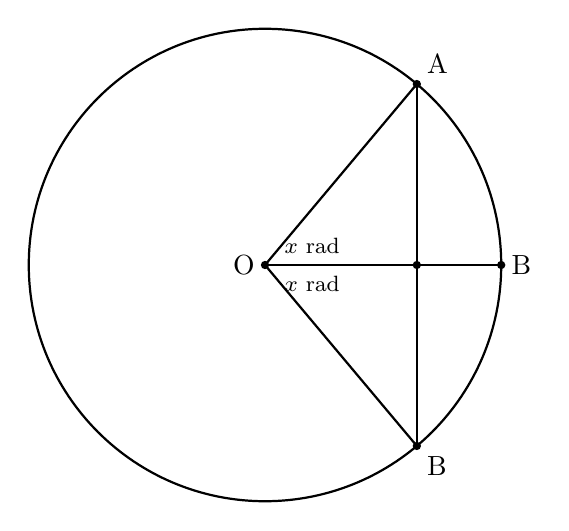
\begin{tikzpicture}[thick, >=stealth, scale=3]
        \coordinate (O) at (0,0);
        \coordinate (B_axis) at (1,0); % Point B on the horizontal axis
        \coordinate (A) at (50:1);    % Point A at 50 degrees
        \coordinate (B_lower) at (-50:1); % Point B at -50 degrees
        \draw (O) circle (1);
        \draw (O) -- (B_axis);
        \draw (O) -- (A);
        \draw (O) -- (B_lower);
        \draw (A) -- (B_lower);
        \fill (O) circle (0.5pt) node[left] {O};
        \fill (A) circle (0.5pt) node[above right] {A};
        \fill (B_axis) circle (0.5pt) node[right] {B};
        \fill (B_lower) circle (0.5pt) node[below right] {B};
        \coordinate (M) at ({cos(50)}, 0);
        \fill (M) circle (0.5pt);
        \node at (0.2, 0.08) {\footnotesize $x$ rad};
        \node at (0.2, -0.08) {\footnotesize $x$ rad};
    \end{tikzpicture} 
\end{center}

The quantity of our interest is the ratio of the length of the chord $AB = 2r\sin x$ to the length of the arc $\overset{\frown}{AB} = 2rx$. Let $y = \frac{2r\sin x}{2rx} = \frac{\sin x}{x}$. Specifically, we are interested in the value of $y$ as $x\to 0$. 

\begin{center}
\begin{tabular}{|c|c|c|c|c|}
\hline
$x=$ & $0.5$ & $0.1$ & $0.05$ & $0.01$ \\
\hline
$y=$ & $0.96$ & $0.998$ & $0.9996$ & $0.99998$ \\
\hline
\end{tabular}
\end{center}
Numerically, we can see from the table as $y \,\xrightarrow{x \to 0}{1}$, then this is our best guess $\lim\limits_{x\to 0}\frac{\sin x}{x} = 1$.

\begin{definition}{\quad The Limit of a Function}{def_4_1_1}
    A function $f(x)$ is well defined on the open interval $O(x_{0}, \rho)\backslash x_{0}$. If $\,\forall\, \epsilon > 0$, there exists $\delta > 0$ such that for all $x$ satisfying
    
    \[
        0 < \vert x - x_{0}\vert < \delta \implies \vert f(x) - A \vert < \epsilon,
    \]
    
    then we say that the \textbf{limit of} $\boldsymbol{f(x)}$, as $x$ approaches $x_{0}$, is $A$, denoted as $\lim\limits_{x\to x_{0}}f(x) = A$. Otherwise, we say that the limit of $f(x)$, as $x$ approaches $x_{0}$, does not exist. 

    \begin{remark}
        Mathematically it is saying 
        \[
        \forall\, \epsilon > 0, \exists\, \delta > 0, \quad \forall\,x  \underbrace{\left(0 < \vert x-x_{0}\vert < \delta\right)}_{x \text{ lives
        in the Punctured } \delta\text{-neighbourhood of }x_{0}} \implies \underbrace{\vert f(x) - f(x_{0}) \vert < \epsilon}_{f(x) \text{ is not too far away from } f(x_{0})} .
        \]
    \end{remark}
    
\end{definition}

\begin{note}
    Here, $O(x_{0}, \rho) = (x_{0}-\rho, x_{0}+\rho)$. In the above Definition \ref{:def_4_1_1}, $f(x)$ does not have to be defined on $x_{0}$.
\end{note}

\begin{definition}{\quad The $\delta$-Neighborhood of $x_{0}$}{def_4_1_2}
    The \textbf{$\boldsymbol{\delta}$-neighborhood of} $\boldsymbol{x_{0}}$ is $O(x_{0}, \delta) \iff \vert x-x_{0}\vert < \delta$.
    \begin{remark}
        Think about whey the two expression are equivalent.
    \end{remark}
\end{definition}

\begin{definition}{\quad The Punctured $\delta$-Neighborhood of $x_{0}$}{def_4_1_3}
    The \textbf{punctured $\boldsymbol{\delta}$-neighborhood of} $\boldsymbol{x_{0}}$ is $O(x_{0}, \delta)\backslash x_{0} \iff 0 < \vert x- x_{0}\vert < \delta$.
    \begin{remark}
        Think about whey the two expression are equivalent.
    \end{remark}
\end{definition}

\begin{example}{\quad}{exp_4_1_1}
    Use the definiton of the limit of a function to prove $\lim\limits_{x\to0}e^{x} = 1$ . 
\end{example}

\begin{proof}{MyExpColor}
[Hint]: In the limit, $x$ approaches $0$. So we know $x$ lives in the punctured $\delta$-neighborhood of $0$. \uwave{For all $\epsilon >0$}, we need to find a $\delta > 0$ such that $\forall\, x \left(0 < \vert x - 0\vert < \delta \right) \implies \vert e^{x} - 1 \vert < \epsilon$.

To find $\delta$, again we need to work the back way around.
    \begin{align*}
        \vert &e^{x} - 1 \vert < \epsilon \\
        -\epsilon <\,\, &e^{x} - 1 < \epsilon \\
        1 - \epsilon <\,\, &e^{x} < \epsilon + 1 \\
        \ln (1-\epsilon) <\,\, &x < \ln (1+\epsilon)
    \end{align*}
    So, \uwave{we find $\delta = \min\left\{ \ln\frac{1}{1-\epsilon}, \ln(1+\epsilon)\right\}$}.

    \begin{note}
        Here, $\ln(1-\epsilon)$ is negative, but the $\delta$, we want, has to be positive. Since $\ln(1-\epsilon) = -\ln\frac{1}{1-\epsilon}$ and indeed $\ln\frac{1}{1-\epsilon}$ is positive.
    \end{note}

    Therefore, we have shown that \uwave{$\forall\, x \left( 0 < \vert x - 0 \vert < \delta\right)$, we have $\vert e^{x} - 1 \vert < \epsilon$}. We proved $\lim\limits_{x\to0}e^{x} = 1$.
\end{proof}

\begin{example}{}{exp_4_1_2}
    Prove $\lim\limits_{x\to2} x^2 = 4$ using the definition. 
\end{example}

\begin{proof}{MyExpColor}
[Hint]: Where does $x$ live? How to find a \textbf{positive} $\delta$ for all $\epsilon > 0$.

    \uwave{For all $\epsilon > 0$}, we need to find a positive $\delta$ such that  $\forall\,x$ in punctured $\delta$-neighborhood of $2$, $x^{2}$ will not be too far away from $4$. 
    
    Again, we work backward to find a $\delta$.
    \begin{align*}
        \vert x^{2} - 4 \vert = 
        \vert (x-2)(x+2)\vert =
        \vert x-2 \vert \cdot \vert x+2 \vert \textcolor{red}{\,<\,}
        \vert x -2\vert \cdot 5 < \epsilon \implies \vert x - 2 \vert < \frac{\epsilon}{5}
    \end{align*}
    
    \uwave{We find $\delta = \min \left\{\frac{\epsilon}{5}, 1\right\}$}. \uwave{ $\forall\, x \left(0 < \vert x - 2\vert < \delta\right)$}: \uwave{$\vert x^{2} - 4\vert < 5\vert x-2 \vert < \epsilon$}. Thus, $\lim\limits_{x\to2}x^{2} = 4$.
\end{proof}
\begin{note}
    The red inequality is because $x \in O(2, \delta)\backslash 2$ meaning $x$ will not be too far away from $2$, i.e., $\vert x-2\vert < 1$ , meaning $\vert x+2 \vert < 5$. More importantly, we kee $\vert x - 2 \vert$ but expand $\vert x + 2 \vert$ to $5$, because $\vert x - 2 \vert$ is the $\delta$-neighborhood of $2$, where $x$ lives. 
\end{note}

\begin{note}
    Here, we include $1$ when find $\delta$ is because we used an extra (but valid and reasonable) condition $\vert x-2 \vert < 1$ to expand $\vert x+ 2\vert$ to make it easier for us to find a $\delta$. Remember we just need to find a $\delta$, NOT the best $\delta$.
\end{note}

\begin{remark}
    In Example \ref{:exp_4_1_1}, the $\delta$ we find is indeed the best $\delta$.
\end{remark}

\begin{remark}
    In Example \ref{:exp_4_1_2}, think about why we expand $\vert x+2\vert$ instead of $\vert x-2\vert$.
\end{remark}

\begin{example}{}{exp_4_1_3}
    Prove $\lim\limits_{x\to1}\frac{x(x-1)}{x^{2}-1} = \frac{1}{2}$.
\end{example}
    \begin{proof}{MyExpColor}
    \uwave{For all $\epsilon > 0$}, we need to find a positive $\delta$ such that  $\forall\,x \left(0 < \vert x-1 \vert< \delta\right)$ we have $\left\vert \frac{x(x-1)}{x^{2}-1} - \frac{1}{2}\right\vert < \epsilon$. We work backwards to find $\delta$.
    \begin{align*}
        \left\vert \frac{x(x-1)}{x^{2}-1} - \frac{1}{2}\right\vert &=
        \left\vert \frac{2x(x-1)-x^{2}+1}{2(x^{2}-1)}\right\vert \\
        &=
        \left\vert \frac{x^{2}-2x+1}{2(x^{2}-1)}\right\vert =
        \frac{\left\vert x-1\right\vert}{ 2\left\vert x+1\right\vert} \textcolor{red}{\,<\,} \frac{\vert x-1\vert}{2} < \epsilon
    \end{align*}
    
    \uwave{We find $\delta = \min\left\{\frac{\epsilon}{2}, 1 \right\}$}. That is \uwave{$\forall\, \left(0 < \vert x-1\vert < \delta\right)$}, \uwave{we have $\left\vert \frac{x(x-1)}{x^{2}-1} - \frac{1}{2}\right\vert < \frac{\vert x-1\vert}{2} < \epsilon$}. So, we proved $\lim\limits_{x\to1}\frac{x(x-1)}{x^{2}-1} = \frac{1}{2}$. Obviously, the $\delta$ we found is not the best one and it does not have to be.
\end{proof}

\begin{note}
    The red inequality is because an extra but reasonable condition $\vert x-1\vert< 1 \iff \vert x+1\vert > 1$.
\end{note}

\begin{remark}
    In Example \ref{:exp_4_1_3}, think about why we expand $\vert x+1\vert$ instead of $\vert x-1\vert$.
\end{remark}



\section{The Properties of the Limits of Functions}\label{sec:4.2}
\subsection{The Uniqueness of the Limit of a Function}

\begin{theorem}{\quad The Uniqueness of the Limit of a Function (at a given point)}{thm_4_2_1}
    Suppose both $A$ and $B$ are limits of $f(x)$ at $x_{0}$, then $A=B$.
\end{theorem}

\begin{proof}{MyThmColor}
    Since we are given that both $A$ and $B$ are limits to $f(x)$ at $x_{0}$, that is
    \begin{align*}
        \text{For all } \epsilon >0, &\,\exists\, \delta_{1} >0, \forall\,x  \left( 0 < \vert x-x_{0}\vert < \delta_{1}\right): \vert f(x) - A \vert < \frac{\epsilon}{2} \\
        &\,\exists\, \delta_{2} >0, \forall\,x  \left(0 < \vert x-x_{0}\vert < \delta_{2}\right): \vert f(x) - B \vert < \frac{\epsilon}{2} \\
    \end{align*}
    We find $\delta = \min\left\{\delta_{1},\delta_{2}\right\}$. We observe
    \begin{align*}
        \vert A - B \vert = \vert A-B + f(x) - f(x)  \vert &= \vert f(x)-B + A - f(x) \vert \\
         &\leq \vert f(x) - B\vert + \vert f(x) -A\vert \\
         &< \frac{\epsilon}{2} + \frac{\epsilon}{2} \\
         &= \epsilon.
    \end{align*}
    Therefore, we have shown $A=B$.
\end{proof}



\subsection{The Local Order-Preserving Property of a Limit of a Function}

\begin{theorem}{\quad}{thm_4_2_2}
    Suppose $\lim\limits_{x\to x_{0}}f(x) = A$, $\lim\limits_{x\to x_{0}}g(x) = B$, and $A > B$. Then $\exists\, \delta > 0$, when $0 < \vert x-x_{0}\vert < \delta$, we have $f(x) > g(x)$.
\end{theorem}

\begin{proof}{MyThmColor}
    Let $\epsilon_{0} = \frac{A-B}{2}$.
    \begin{align*}
        \lim\limits_{x\to x_{0}}f(x) = A:\quad \exists\, \delta_{1}, \forall\,x  \left(0 < \vert x-x_{0}\vert < \delta_{1}\right): \vert f(x) - A\vert < \epsilon_{0} \implies f(x) > A - \epsilon_{0} = \frac{A+B}{2}. \\
        \lim\limits_{x\to x_{0}}g(x) = B:\quad \exists\, \delta_{2}, \forall\,x  \left(0 < \vert x-x_{0}\vert < \delta_{2}\right): \vert g(x) - B\vert < \epsilon_{0} \implies g(x) < B + \epsilon_{0} = \frac{A+B}{2}.
    \end{align*}
    Let $\delta = \min\left\{\delta_{1}, \delta_{2}\right\}$, we have shown that $\forall\,x  \left(0<\vert x - x_{0}\vert < \delta\right)$, we have $f(x) > \frac{A+B}{2}> g(x)$.
\end{proof}

\begin{corollary}{\quad}{cor_4_2_3}
    Suppose $\lim\limits_{x\to x_{o}}f(x) = A \neq 0$, then $ \exists\, \delta >0$ when $0 < \vert x-x_{0} \vert < \delta$ we have $\vert f(x)\vert > \frac{\vert A \vert}{2} > 0$.
\end{corollary}
\begin{proof}{MyCorColor}
    Since $\lim\limits_{x\to x_{0}}f(x) = A$, we have $\forall\, \epsilon > 0, \exists\, \delta > 0, \forall\,x  \left(0 < \vert x -x_{0}\vert < \delta\right): \vert f(x) - A \vert< \epsilon$. Note we also have 
    \begin{align*}
        \vert f(x)\vert - \vert A\vert &\leq \vert f(x) - A\vert \\
        \Big\vert\vert f(x)\vert - \vert A\vert\Big\vert &\leq \vert f(x) - A\vert
    \end{align*}
    That is $\forall\, \epsilon > 0, \exists\, \delta > 0, \forall\,x  \left(0 < \vert x -x_{0}\vert < \delta\right): \Big\vert\vert f(x)\vert - \vert A\vert\Big\vert < \epsilon$. We have shown $\lim\limits_{x\to x_{0}} \vert f(x)\vert = \vert A\vert$. 

    Let $g(x) = \frac{\vert A\vert}{2}$, it is obvious that $\vert A \vert > \frac{\vert A\vert}{2}$. By Theorem \ref{:thm_4_2_2}, we have that $ 0 < \vert x-x_{0}\vert < \delta: \vert f(x)\vert > g(x) = \frac{\vert A\vert}{2}$.
\end{proof}

\begin{remark}
    The converse of Theorem \ref{:thm_4_2_2} is incorrect. That is suppose $\lim\limits_{x\to x_{0}}f(x) = A$, $\lim\limits_{x\to x_{0}}g(x) = B$, and $\exists\, \delta > 0$, $0 < \vert x-x_{0}\vert < \delta$, if $f(x) > g(x) \centernot \implies A > B$. A counter example is $f(x) = 2x^{2}, g(x) = x^{2}$ and $x_{0} = 0$. It is obvious that in the punctured $\delta$-neighborhood of $0$, we do have $f(x) > g(x)$, but $A = B$. So, the puncture $\delta$-neighborhood is the key. Next we give a valid converse of Theorem \ref{:thm_4_2_2}.
\end{remark}

\begin{corollary}{\quad}{cor_4_2_4}
    Suppose $\lim\limits_{x\to x_{0}}f(x) = A$, $\lim\limits_{x\to x_{0}}g(x) = B$. If $\exists\, \delta > 0$, for $0 < \vert x-x_{0}\vert < \delta$ such that $f(x) > g(x)$, then $ A \geq B$.
\end{corollary}
\begin{proof}{MyCorColor}
    If $A < B$, then 
    
    \[
    \exists\, \delta_{1} > 0, \forall\,x  \left(0 \vert x-x_{0} \vert < \delta_{1}\right): f(x) < g(x).
    \]
    
    Now, let $\delta^{*} = \min\left\{\delta, \delta_{1}\right\}$, $\forall\,x  \left(0 < \vert x-x_{0} \vert < \delta^{*}\right): f(x) \geq g(x) \text{ and } f(x) < g(x)$. Contradiction.
\end{proof}



\subsection{The Local Boundedness Property of a Limit of a Function}

\begin{theorem}{\quad}{thm_4_2_5}
    Suppose $\lim\limits_{x\to x_{0}}f(x) = A$, then 
    \begin{align*}
        \exists\, \delta > 0, \forall\,x  \left(0 < \vert x - x_{0}\vert < \delta\right): m \leq f(x) \leq M,
    \end{align*}
    with $m$, and $M$ are two fixed real numbers.
\end{theorem}

\begin{proof}{MyThmColor}
    W.O.L.G., let $m \leq A \leq M$, and let $g(x) = m$ and $h(x) = M$. Immediately, we have $\lim\limits_{x\to x_{0}}g(x) = m$ and $\lim\limits_{x\to x_{0}}h(x) = M$, since both $g(x)$ and $h(x)$ are constant functions. Then by Theorem \ref{:thm_4_2_2}, 
    
    \begin{align*}
        \exists\, \delta >0, \forall\,x  \left(0 < \vert x-x_{0}\vert < \delta\right): m = g(x) < f(x) < h(x) = M.
    \end{align*}
\end{proof}

\begin{remark}
    If $f(x)$ is defined at $x_{0}$, then $\vert x-x_{0}\vert < \delta: \min\left\{m, f(x_{0})\right\}\leq f(x) \leq \max\left\{M, f(x_{0})\right\}$.
\end{remark}



\subsection{The Squeeze Theorem}
\begin{theorem}{\quad The Squeeze Theorem}{thm_4_2_6}
    Suppose $\exists\,r > 0, \forall\,x  \left(0 < \vert x-x_{0}\vert  < r\right), g(x) \leq f(x) \leq h(x)$ and $\lim\limits_{x\to x_{0}}g(x) = \lim\limits_{x\to x_{0}}h(x) = A$, then $\lim\limits_{x\to x_{0}}f(x) = A$.
\end{theorem}

\begin{proof}{MyThmColor}
    Immediately, we have
    \begin{align*}
        \uwave{\forall\, \epsilon > 0}, &\,\exists\,\delta_{1}> 0, \forall\,x  \left(0 < \vert x-x_{0}\vert < \delta_{1}\right): \vert g(x) - A \vert < \epsilon \implies g(x) > A - \epsilon \implies -\epsilon < g(x) - A. \\
        &\,\exists\,\delta_{2} > 0, \forall\,x  \left(0 < \vert x-x_{0}\vert < \delta_{2}\right): \vert h(x)-A\vert <\epsilon \implies h(x) < A + \epsilon \implies h(x) -A < \epsilon.
    \end{align*}
    \uwave{We find $\delta = \min\left\{r, \delta_{1},\delta_{2}\right\}$}, \uwave{$\forall\,x  \left(0 < \vert x-x_{0}\vert < \delta\right):$} $g(x) \leq f(x) \leq h(x) \implies g(x)-A \leq f(x)-A \leq h(x)-A$, then $-\epsilon < f(x)-A < \epsilon$ $\implies$ \uwave{$\vert f(x) - A \vert < \epsilon$}. Thus, we proved $\lim\limits_{x\to x_{0}}f(x) = A$.
\end{proof}

\begin{note}
    The Theorem \ref{:thm_4_2_6} is extremely useful when the limit of $f(x)$ is difficult to find, but we observe that if we loose and expand $f(x)$ to $g(x)$ and $h(x)$, respectively, whose limits are the same and easy to find.
\end{note}

\begin{example}{\quad}{exp_4_2_1}
    Prove $\lim\limits_{x\to 0}\frac{\sin x}{x} = 1$. 
    \begin{center}
        \begin{tikzpicture}[>=stealth, scale=4]
            % Draw axes
            \draw[->] (-0.2,0) -- (1.3,0) node[right] {$x$};
            \draw[->] (0,-0.2) -- (0,1.2) node[above] {$y$};
            \coordinate (O) at (0,0);
            \coordinate (B) at (1,0);
            \coordinate (A) at (30:1); % Angle x is set to 30 degrees for 
            \coordinate (C) at (1, {tan(30)});
            \draw[thick] (1,0) arc (0:90:1);
            \draw[thick] (O) -- (A);   % Line OC
            \draw[thick] (O) -- (B);   % Line OB
            \draw[thick] (A) -- (B);   % Chord AB
            \draw[dashed] (B) -- (C);  % Vertical line BC (tan x)
            \draw[dashed] (A) -- (C);  
            \node[below left] at (O) {$O$};
            \node[above right] at (B) {$B$};
            \node[left] at (A) {$A$};
            \node[above] at (C) {$C$};
            \node[left] at (0,1) {$1$};
            \node[below] at (1,0) {$1$};
            \draw (0.2,0) arc (0:30:0.2);
            \node at (15:0.3) {$x$};
        \end{tikzpicture}
    \end{center}
\end{example}
    
\begin{proof}{MyExpColor}
    From the graph, it is obvious that $S_{\triangle 0AB} < S_{\stackrel{\frown}{ABC}} < S_{\triangle OBC}$. That is
    \begin{align*}
        \frac{1}{2}\sin x &< \frac{1}{2}x < \frac{1}{2}\tan x, x\in (0, \frac{\pi}{2}), x \text{ in radius}, \\
        \implies \sin x &< x < \tan x, \\
        \implies \frac{\sin x}{x} &< 1, \text{ and } \cos x < \frac{\sin x}{x}, \\
        \implies \cos x &< \frac{\sin x}{x} < 1.
    \end{align*}
    By the Squeeze Theorem (Theorem \ref{:thm_4_2_6}), we immediately have $\lim\limits_{x\to 0}\frac{\sin x}{x} = 1$, since $\lim\limits_{x\to 0} \cos x = 1$.
    \begin{note}
        In this proof, it still remains to show that $\lim\limits_{x\to 0} \cos x = 1$, which is left as an exercise.
    \end{note}
\end{proof}



\section{The Arithmetic Operations on Limits of Functions}\label{sec:4.3}

\begin{theorem}{\quad}{thm_4_3_1}
    Suppose $\lim_{x \to x_0} f(x) = A$ and $\lim_{x \to x_0} g(x) = B$. Then:
    
    \begin{align*}
        &1) \quad \lim_{x \to x_0} (\alpha f(x) + \beta g(x)) = \alpha A + \beta B; \\
        &2) \quad \lim_{x \to x_0} (f(x)g(x)) = AB; \\
        &3) \quad \lim_{x \to x_0} \frac{f(x)}{g(x)} = \frac{A}{B}, B \neq 0.
    \end{align*}
\end{theorem}

\begin{proof}{MyThmColor}
    From $\lim\limits_{x\to x_{0}}f(x) = A$, we have: 
    \begin{align*}
        &\exists\, \delta_{0} > 0, \forall\,x  \left(0< \vert x-x_{0} \vert < \delta_{0}\right): f(x) \leq X. \\
        \forall\, \epsilon, \,&\exists\, \delta_{1} > 0, \forall\,x  \left(0 < \vert x-x_{0}\vert < \delta_{1}\right): \vert f(x) - A \vert < \epsilon.
    \end{align*}
    From $\lim\limits_{x\to x_{0}}g(x) = B$, we have: 
    \begin{align*}
        \forall\, \epsilon, \,&\exists\, \delta_{2} > 0, \forall\,x  \left(0 < \vert x-x_{0}\vert < \delta_{2}\right): \vert g(x) - B \vert < \epsilon.
    \end{align*}
    
    To prove $1)$ in Theorem \ref{:thm_4_3_1}, we find $\delta = \min\left\{\delta_{0}, \delta_{1}, \delta_{2} \right\}, \forall\,x  \left(0 < \vert x- x_{0}\vert < \delta\right)$, we need to show:
    \[
    \left\vert \alpha f(x) + \beta g(x) - (\alpha A + \beta B)\right\vert < \epsilon.
    \]
    We start from the LHS.
    \begin{align*}
        \left\vert \alpha f(x) + \beta g(x) - (\alpha A + \beta B)\right\vert &= \left\vert \alpha \big(f(x)-A\big) + \beta \big(g(x) -B\big)\right\vert \\
        &\leq \vert \alpha\vert\left\vert f(x) -A \right\vert + \vert\beta\vert\left\vert g(x) - B\right\vert \\
        &< \left(\vert \alpha \vert + \vert \beta \vert\right)\epsilon
    \end{align*}
    We have proved $1)$ in Theorem \ref{:thm_4_3_1}. 

    To prove $2)$ from Theorem \ref{:thm_4_3_1}, we find $\delta = \min\left\{\delta_{0}, \delta_{1}, \delta_{2} \right\}, \forall\,x  \left(0 < \vert x- x_{0}\vert < \delta\right)$, we need to show $\vert f(x)g(x) - AB \vert < \epsilon$.
    \begin{align*}
        \left\vert f(x)g(x) - AB\right\vert  &= \left\vert f(x)g(x) \textcolor{blue}{-Bf(x) + Bf(x)} - AB\right\vert \\ 
        &= \left\vert f(x) \big(g(x)-B\big) + B\big(f(x) -A\big)\right\vert \\
        & \leq \left\vert f(x) \right\vert \left\vert g(x)-B\right\vert + \left\vert B \right\vert \left\vert f(x) -A\right\vert \\
        &< \big(\left\vert f(x) \right\vert + \left\vert B\right\vert\big)\epsilon \\
        &< \left( X + \vert B\vert\right)\epsilon
    \end{align*}
    We have proved $2.)$ in Theorem \ref{:thm_4_3_1}. 

    To prove $3)$ in Theorem \ref{:thm_4_3_1}, we find $\delta = \min\left\{\delta_{0}, \delta_{1}, \delta_{2} \right\}, \forall\,x  \left(0 < \vert x- x_{0}\vert < \delta\right)$, we need to show $\left\vert \frac{f(x)}{g(x)} - \frac{A}{B}\right\vert < \epsilon$. By Corollary \ref{:cor_4_2_3}, we know $\exists\,\delta^{*}> 0, \forall\,x  \left(0 < \vert x-x_{0} \vert < \delta^{*}\right): \vert g(x)\vert > \frac{\vert B\vert}{2}$.
    \begin{align*}
        \left\vert \frac{f(x)}{g(x)} - \frac{A}{B}\right\vert &= \frac{\left\vert Bf(x) \textcolor{blue}{-AB + AB} - Ag(x)\right\vert}{\vert B g(x)\vert} \\
        &= \frac{\left\vert B\big(f(x) -A\big) + A\big(B - g(x)\big)\right\vert}{\vert B g(x)\vert} \\
        &\leq \frac{\left(\vert B\vert +\vert A\vert\right)\epsilon}{\vert B\vert\vert g(x)\vert} \\
        &< 2\frac{\vert B\vert +\vert A\vert}{\vert B\vert^{2}} \epsilon
    \end{align*}
    We have proved $3)$ in Theorem \ref{:thm_4_3_1}.
\end{proof}

\begin{example}{\quad}{exp_4_3_1}
    For $\alpha \neq 0$, $\lim\limits_{x\to 0}\frac{\sin \alpha x}{x} = \alpha\lim\limits_{x\to 0}\frac{\sin \alpha x}{\alpha x} = \alpha$.
\end{example}

\begin{example}{\quad}{exp_4_3_2}
    For $\alpha \neq 0, \beta\neq0$, $\lim\limits_{x\to0}\frac{\sin \alpha x}{\sin \beta x} = \lim\limits_{x\to0} \frac{\alpha x}{\beta x}\frac{\frac{\sin \alpha x}{\alpha x}}{\frac{\sin \beta x}{\beta x}} = \frac{\alpha x}{\beta x} = \frac{\alpha}{\beta}$.
\end{example}



\section{The Relationship Between the Limit of a Function and the Limit of a Sequence}
\subsection{The Mathematical Analysis Expression of the Negation Proposition}
Before we dive into the main content for this chapter, we need to make sure that we know how to express the \textbf{negation} of a given proposition in mathematical analysis way. 

The proposition $P$: 

A sequence $\left\{x_{n}\right\}$ converges to $a$: $\quad\quad\quad\quad\forall\,\epsilon >0, \,\exists\,N, \forall\, n > N: \vert x_{n} - a\vert < \epsilon$. 

It's \textbf{negation} is $\neg P$: 

A sequence $\left\{x_{n}\right\}$ does not converge to $a$: $\quad \exists\,\epsilon>0, \forall\, N, \,\exists\,n > N : \vert x_{n} - a\vert \geq \epsilon$. 



\subsection{The Heine Theorem}
The Heine theorem provides a crucial link between the limit of a function and the limit of a sequence, offering an alternative way to define and understand function limits using sequences.

\begin{theorem}{\quad The Heine Theorem}{thm_4_4_1}
    The necessary and sufficient condition for $\lim\limits_{x\to x_{0}}f(x) = A$ is that for \textcolor{red}{any arbitrary} sequence $\left\{x_{n}\right\}$ satisfies $x_{n} \neq x_{0}$ and $\lim\limits_{n\to\infty}x_{n} = x_{0}$, the sequence $\left\{f(x_{n})\right\}$ converges to $A$.
\end{theorem}

\begin{proof}{MyThmColor}
    $(\Rightarrow)$. Given $\lim\limits_{x\to x_{0}}f(x) = A$, we have 
    \[
        \uwave{\forall\,\epsilon >0}, \,\exists\, \delta > 0, \forall\,x  \left(0 < \vert x-x_{0}\vert < \delta\right): \vert f(x) -A \vert <\epsilon.
    \]
    Give $\lim\limits_{n\to\infty}x_{n} = x_{0}$, we have
    \[
        \forall\,\delta > 0, \uwave{\,\exists\, N > 0}, \uwave{\forall\, n > N}: 0 < \vert x_{n} - x_{0}\vert < \delta.
    \]
    Therefore, we have \uwave{$\vert f(x_{n}) - A\vert < \epsilon$}, that is $\lim\limits_{n\to\infty}f(x_{n}) = A$. 

    $(\Leftarrow)$. We will use \textbf{proof by contrapositive} to prove the sufficient condition. 
    
    The sufficient condition $(\Leftarrow)$, call it $S$, is: 
    
    For any sequence $\left\{x_{n}\right\}$ satisfies $x_{n} \neq x_{0}, \lim\limits_{n\to\infty}x_{n} = x_{0}$, and the sequence $\left\{f(x_{n})\right\}$ converges to $A$, \textbf{ then } $\lim\limits_{x\to x_{0}}f(x) = A$. 

    It's \textbf{contrapositive}, $\neg S$, is: 
    
    If $\lim\limits_{x\to x_{0}}f(x) \neq A$, \textbf{then} for any sequence $\left\{x_{n}\right\}$ satisfies $x_{n} \neq x_{0}, \lim\limits_{n\to\infty}x_{n} = x_{0}$, the sequence $\left\{f(x_{n})\right\}$ does NOT converge to $A$. 

    Now, we just need to prove the \textbf{contrapositive}. We write the contrapositive in the mathematical analysis expression. 

    \textcolor{gray}{$\lim\limits_{x\to x_{0}}f(x) \neq A$:} $\quad\quad\quad \exists\,\epsilon_{0}>0, \forall\,\delta > 0, \forall\, x \left(0< \vert x - x_{0}\vert < \delta\right): \vert f(x) - A\vert \geq \epsilon_{0}$. 

    Let $\delta_{n} =\frac{1}{n}$, this is for the sake of $\frac{1}{n} \,\xrightarrow{n \to \infty} 0$: 
    
    \begin{align*}
        \delta_{1} = 1: \quad &\exists\,x_{1}, 0< \vert x_{1} - x_{0}\vert < \delta_{1}: \vert f(x_{1}) - A\vert \geq \epsilon_{0}, \\
        \delta_{2} = \frac{1}{2}: \quad &\exists\,x_{2}, 0< \vert x_{2} - x_{0}\vert < \delta_{2}: \vert f(x_{2}) - A\vert \geq \epsilon_{0}, \\
        \vdots \\
        \delta_{3} = \frac{1}{3}: \quad &\exists\,x_{2}, 0< \vert x_{3} - x_{0}\vert < \delta_{3}: \vert f(x_{2}) - A\vert \geq \epsilon_{0}, \\
        \vdots \\
        \delta_{k} = \frac{1}{k}: \quad &\exists\,x_{2}, \underbrace{0< \vert x_{k} - x_{0}\vert < \delta_{k}=\frac{1}{k}:}_{x_{n}\,\xrightarrow{n \to \infty\,} x_{0}} \vert f(x_{k}) - A\vert \geq \epsilon_{0}, \\
        \vdots
    \end{align*}
    We find a sequence $\left\{x_{n}\right\}$, $x_{n} \neq x_{0}$, $\lim\limits_{n\to\infty}x_{n} = x_{0}$, but $\left\{f(x_{n})\right\}$ does not converge to $A$. We have prove the \textbf{contrapositive}, $\neg S$, so the proposition $S$ is true.
\end{proof}

\begin{remark}
    The Heine Theorem \ref{:thm_4_4_1} tells us that finding only one sequence $\left\{x_{n}\right\}, x_{n} \neq x_{0}, \lim\limits_{n\to\infty}x_{n}=x_{0}$ and the sequence $\left\{f(x_{n})\right\}$ converges to $A$ is not enough to show $\lim\limits_{x\to x_{0}}f(x) = A$.  
\end{remark}

\begin{example}{\quad}{exp_4_4_1}
    Find the limit of $\sin \frac{1}{x}$ at $x_{0} = 0$.
\end{example}

\begin{proof}{MyExpColor}
    We pick the fist sequence $\left\{x_{n}^{(1)}\right\}$: 
    \begin{align*}
        x_{n}^{(1)} = \frac{1}{n\pi}, x_{n} \neq x_{0}, \lim\limits_{n\to\infty}x_{n} = x_{0}=0: \lim\limits_{x\to\infty}\sin \frac{1}{x_{n}^{(1)}} = \lim\limits_{x\to\infty}\sin n\pi = 0.
    \end{align*}
    
    We pick the second sequence $\left\{x_{n}^{(2)}\right\}$:
    \begin{align*}
        x_{n}^{(2)} =\frac{1}{2n\pi + \frac{\pi}{2}}, x_{n} \neq x_{0}, \lim\limits_{n\to\infty}x_{n} = x_{0}=0: \lim\limits_{x\to\infty}\sin \frac{1}{x_{n}^{(2)}} = \lim\limits_{x\to\infty}\sin (2n\pi + \frac{\pi}{2}) = 1.
    \end{align*}

    So, by Heine Theorem \ref{:thm_4_4_1}, we know the limit of $\sin \frac{1}{x}$, at $x_{0}=0$ does not exist.
\end{proof}

\begin{theorem}{}{thm_4_4_2}
    The necessary and sufficient condition for $\lim\limits_{x\to x_{0}}f(x)$ exists and being finite (or converges) is that for \textcolor{red}{any} sequence $\left\{x_{n}\right\}$ satisfies $x_{n} \neq x_{0}$ and $\lim\limits_{n\to\infty}x_{n} = x_{0}$, the sequence $\left\{f(x_{n})\right\}$ converges.
\end{theorem}

\begin{remark}
    Compare Theorem \ref{:thm_4_4_2} with Theorem \ref{:thm_4_4_1}. Actually we do not need to know the limit, we only need to know they converge.
\end{remark}



\section{One-sided Limit}
\begin{definition}{\quad Left-hand Limit}{def_4_5_1}
    Suppose $f(x)$ is defined on $(x_{0}-\rho, x_{0})$. If there exists a $B$, $\forall\, \epsilon>0, \,\exists\, \delta>0, \forall\, x \left( -\delta < x - x_{0} < 0\right): \left\vert f(x) - B\right\vert<\epsilon $. Then, $B$ is called the \textbf{Left-hand Limit} of $f(x)$ at $x_{0}$. Denoted as
    \[
        \lim\limits_{x\to x_{0}^{-}}f(x) = B,\quad \text{ or } \quad f(x) \xrightarrow{x \to x_{0}^{-}}B.
    \]
\end{definition}

\begin{note}
    Here, $\delta$ has to be smaller than $\rho$.
\end{note}

\begin{definition}{\quad Right-hand Limit}{def_4_5_2}
    Suppose $f(x)$ is defined on $(x_{0}, x_{0}+\rho)$. If there exists a $C$, $\forall\, \epsilon>0, \,\exists\, \delta>0, \forall\, x \left( 0 <  x - x_{0} < \delta \right): \left\vert f(x) - C\right\vert<\epsilon $. Then, $C$ is called the \textbf{Right-hand Limit} of $f(x)$ at $x_{0}$. Denoted as
    \[
        \lim\limits_{x\to x_{0}^{+}}f(x) = C,\quad \text{ or } \quad f(x) \xrightarrow{x \to x_{0}^{+}}C.
    \]
\end{definition}

\begin{note}
    Again, $\delta$ has to be smaller than $\rho$.
\end{note}
    
\begin{proposition}{\quad}{prop_4_5_1}
    \[
        \lim\limits_{x\to x_{0}}f(x) = A \quad \Longleftrightarrow \quad\lim\limits_{x\to x_{0}^{-}}f(x) = \lim\limits_{x\to x_{0}^{+}}f(x) = A.
    \]
\end{proposition}

\begin{example}{\quad}{}
    For $\text{sgn} x$,
    \[
        \text{sgn} x = \begin{cases}
            \quad 1, & \text{if } x > 0; \\
            \quad 0, & \text{if } x = 0; \\
            \quad -1, & \text{if } x < 0.
                \end{cases}
    \]
    \[
        \lim\limits_{x \to 0^{-}} \text{sgn} x = -1, \quad \text{ or } \quad \lim\limits_{x \to 0^{+}} \text{sgn} x = 1, 
    \]
\end{example}

\begin{example}{}{exp_4_5_2}
    Find the limit of $f(x)$ at $x_{0}=0$.

\[
    f(x) = \begin{cases}
        \quad \frac{\sin 2x}{x}, & \text{if } x < 0; \\
        \quad 2\cos x^{2}, & \text{if } x \geq 0. 
    \end{cases} 
\]
\end{example}

\begin{solve}{MyExpColor}
    \begin{align*}
        \lim\limits_{x\to 0^{+}}f(x) &= \lim\limits_{x\to 0^{+}} 2\cos x^{2} = 2, \\
        \lim\limits_{x\to 0^{-}}f(x) &= \lim\limits_{x\to 0^{-}} \frac{\sin 2x}{x} = 2
    \end{align*}
    
    Therefore, $\lim\limits_{x\to 0}f(x) = 2$.
\end{solve}



\section{The Extension of the Definition of a Limit of a Function}\label{sec:4.6}

For $\lim\limits_{x\to x_{0}}f(x) = A$, it contains two messages $\textcolor{blue}{x\to x_{0}}$ and $\textcolor{orange}{f(x) \to A}$. 
\[
    \textcolor{orange}{\forall\, \epsilon > 0}, \textcolor{blue}{\,\exists\,\delta>0}, \textcolor{blue}{\,\forall\, x \left(0< \vert x-x_{0}\vert < \delta\right)}, \textcolor{orange}{\vert f(x) - A\vert} < \epsilon.
\]
It is obvious that the blue terms are about $x$ and orange terms about $f(x)$. Since we have introduced left-and right-limits in last section, we know have more mathematical analysis expression for $x$.

\begin{align*}
    x\to x_{0}: &\quad \exists\, \delta >0, \forall\, x,\, (0 < \vert x-x_{0}\vert < \delta); \\
    x\to x^{+}: &\quad \exists\,\delta > 0, \forall\,x,\, (0 < x - x^{+} < \delta); \\
    x\to x^{-}: &\quad \exists\,\delta > 0, \forall\,x,\, (-\delta < x - x^{-} < 0); \\
    x\to+\infty: &\quad \exists\,X>0, \forall\,x,\,(x > X); \\
    x\to-\infty: &\quad \exists\,X>0, \forall\,x,\,(x < -X); \\
    x\to\infty: &\quad \exists\,X>0, \forall\,x,\,(\vert x\vert  > X). \\
\end{align*}
Now, let's look at $f(x)$.
\begin{align*}
    f(x) \to A: &\quad \forall\, \epsilon > 0, \dots, \vert f(x) - A\vert < \epsilon; \\
    f(x) \to +\infty: &\quad \forall\, G > 0, \dots, f(x) > G; \\
    f(x) \to -\infty: &\quad \forall\, G > 0, \dots, f(x) < -G; \\
    f(x) \to \infty: &\quad \forall\, G > 0, \dots, \vert f(x)\vert > G. \\
\end{align*}

\begin{example}{}{exp_4_6_1}
    \begin{align*}
        \lim\limits_{x\to x_{0}}f(x) = \infty: &\quad \forall\,G > 0, \,\exists\,\delta > 0, \,\forall\, x,\, (0 < \vert x-x_{0}\vert < \delta): \vert f(x) \vert > G. \\
        \lim\limits_{x\to+\infty}f(x) = A: &\quad \forall\, \epsilon>0,\,\exists X >0, \,\forall\,x,\, (x > X): \vert f(x) - A \vert < \epsilon. \\
        \lim\limits_{x\to -\infty}f(x) = +\infty: &\quad \forall\, G > 0, \,\exists\, X > 0, \,\forall\,x,\, (x<-X): f(x) >G.
    \end{align*}
\end{example}

\begin{example}{}{exp_4_6_2}
    Prove $\lim\limits_{x\to -\infty}e^{x} = 0$.
\end{example}

\begin{proof}{MyExpColor}
    That is \uwave{$\forall\, \epsilon >0$}, we need to find $X>0, \,\forall\,x,\,(x < -X):$
    \begin{align*}
        \vert e^{x} - 0\vert < \epsilon \Longleftrightarrow 0 < e^{x} < \epsilon \Longleftrightarrow x < \ln \epsilon = -\ln\frac{1}{\epsilon}. 
    \end{align*}
\uwave{We find $X = \ln\frac{1}{\epsilon} >0$}, \uwave{$\forall\,x,\,(x < -X):$} \uwave{$\quad\vert e^{x} - 0\vert < \epsilon$}.
\end{proof}

\begin{example}{}{exp_4_6_3}
    Prove $\lim\limits_{x\to-1}\frac{x^{2}}{x-1} = -\infty$.
\end{example}

\begin{proof}{MyExpColor}
    That is \uwave{$\forall\, G > 0$}, we want to find a $\delta >0, \,\forall\,x,\,(-\delta < x-1<0):$ 
    \begin{align*}
        \frac{x^{2}}{x-1} < \frac{M}{x-1} < -G \Longleftrightarrow x-1 \textcolor{red}{\,>\,} -\frac{M}{G}
    \end{align*}
    \begin{note}
        The red inequality is because $x-1 < 0$. 
    \end{note}
    Now, we only need to \uwave{contract} $x^{2}$ to $M$, again since $x-1 <0$. Let $-\frac{1}{2} < x-1 < 0 \implies x > \frac{1}{2} \implies x^{2} > \frac{1}{4}$. Therefore,
    \begin{align*}
        x-1 \textcolor{red}{\,>\,} -\frac{1}{4G}.
    \end{align*}
    \uwave{We find $\delta = \min\left\{\frac{1}{2}, \frac{1}{4G}\right\}$}, \uwave{$\forall\,x,\, (-\delta < x-1<0)$}:\uwave{$\quad \frac{x^{2}}{x-1} < -G$}. We proved $\lim\limits_{x\to-1}\frac{x^{2}}{x-1} = -\infty$.
\end{proof}

\begin{remark}
    When talking about The Properties of the Limits of Functions (Section \eqref{sec:4.2}), we were talking about 
    \[
        \lim\limits_{x\to x_{0}}f(x) = A.
    \]
    Since we have now extended $A$ to $-\infty,+\infty,\infty$, we need to be careful with $\infty$. Specifically, the Local Order-Preserving Property (Theorem \ref{:thm_4_2_2}) and the Squeeze Theorem \ref{:thm_4_2_6} works for all situations \uwave{except} for $\infty$.
\end{remark}

\begin{remark}
    When talking about The Arithmetic Operations on Limits of Functions (Section \eqref{sec:4.3}), the arithmetic operations do not apply to the \textbf{indeterminate forms} in function limit operations.
\end{remark}

\begin{example}{}{exp_4_6_4}
    To rewrite the Heine Theorem \ref{:thm_4_4_1}, with $-\infty, +\infty,\infty$ included:
    \begin{align*}
        \lim\limits_{x\to+\infty}f(x) =A &\Longleftrightarrow \text{ For any } \left\{x_{n}\right\}, x_{n}\xrightarrow{n\to+\infty}+\infty: \left\{f(x_{n})\right\} \text{ converges to } A. \\
        \lim\limits_{x\to+\infty}f(x) \text{ exists and converges} &\Longleftrightarrow \text{ For any } \left\{x_{n}\right\}, x_{n}\xrightarrow{n\to+\infty}+\infty: \left\{f(x_{n})\right\} \text{ converges}.\\
    \end{align*}
\end{example}

\begin{example}{}{exp_4_6_5}
    Given $f(x) = \frac{a_{n}x^{n} + a_{n-1}x^{n-1} + \,\dots\, + a_{k}x^{k}}{b_{m}x^{m} + b_{m-1}x^{m-1} + \,\dots\, + b_{j}x^{j}}$, with $a_{n}, a_{k},b_{m},b_{j} \neq 0$. Find $\lim\limits_{x\to \infty}f(x)$ and $\lim\limits_{x\to 0}f(x)$.
\end{example}

\begin{solve}{MyExpColor}
    $(x \to \infty)$ 
    \begin{enumerate}
        \item [i.)] $n=m$:
        \[
            f(x) = \frac{a_{n} + a_{n-1}\frac{1}{x} + \,\dots\, + a_{k}\frac{1}{x^{n-k}}}{b_{m} + b_{m-1}\frac{1}{x} + \,\dots\, + b_{j}\frac{1}{x^{m-j}}} \implies \lim\limits_{x\to\infty}f(x) = \frac{a_{n}}{b_{m}},
        \]
        \item [ii.)] $n > m$:
        \[
            f(x) = x^{n-m}\cdot\frac{a_{n} + a_{n-1}\frac{1}{x} + \,\dots\, + a_{k}\frac{1}{x^{n-k}}}{b_{m} + b_{m-1}\frac{1}{x} + \,\dots\, + b_{j}\frac{1}{x^{m-j}}} \implies \lim\limits_{x\to\infty}f(x) = \infty,
        \]
        \item [iii.)] $n<m$:
        \[
            f(x) = \frac{1}{x^{m-n}}\cdot\frac{a_{n} + a_{n-1}\frac{1}{x} + \,\dots\, + a_{k}\frac{1}{x^{n-k}}}{b_{m} + b_{m-1}\frac{1}{x} + \,\dots\, + b_{j}\frac{1}{x^{m-j}}} \implies \lim\limits_{x\to\infty}f(x) = 0.
        \]
    \end{enumerate}
    $(x\to0)$
    \begin{enumerate}
        \item [i.)] $k=j$:
        \[
            f(x) = \frac{a_{n}x^{n-j} + a_{n-1}x^{n-j-1} + \,\dots\, + a_{k}}{b_{m}x^{m-j} + b_{m-1}x^{m-j-1} + \,\dots\,+ b_{j}} \implies \lim\limits_{x\to0}f(x) = \frac{a_{k}}{b_{j}},
        \]
        \item [ii.)] $k>j$:
        \[
            f(x) = \frac{a_{n}x^{n-k} + a_{n-1}x^{n-k-1} + \,\dots\, + a_{k}}{b_{m}x^{m-j} + b_{m-1}x^{m-j-1} + \,\dots\,+ b_{j}} x^{k-j}\implies \lim\limits_{x\to0}f(x) = 0,
        \]
        \item [iii.)] $k<j$:
        \[
            f(x) = \frac{a_{n}x^{n-k} + a_{n-1}x^{n-k-1} + \,\dots\, + a_{k}}{b_{m}x^{m-j} + b_{m-1}x^{m-j-1} + \,\dots\,+ b_{j}} \frac{1}{x^{j-k}}\implies \lim\limits_{x\to0}f(x) = \infty.
        \]
    \end{enumerate}
\end{solve}
    
\begin{note}
    This example tells us that when $x\to\infty$ the dominant terms are $x$ with the highest exponent, while $x\to0$ the dominant terms are $x$ with the lowest exponent.
\end{note}

\begin{example}{}{exp_4_6_6}
    Show that $\lim\limits_{x\to\infty}\left(1 + \frac{1}{x}\right)^{x} = e$.
\end{example}

\begin{solve}{MyExpColor}
    We have prove the limit of the sequence $\lim\limits_{n\to\infty}\left(1+\frac{1}{n}\right)^{n} = e$. We \uwave{cannot} use the Heine Theorem \ref{:thm_4_4_1} here just because only one sequence $\left\{x_{n} = 1+ \frac{1}{n}\right\}$ converges to $e$. We will use the Squeeze Theorem \ref{:thm_4_2_6}. 

    First, we show that $\lim\limits_{x\to+\infty}\left(1+\frac{1}{x}\right)^{x} = e$. Since $\forall\, x\geq 1$ we have $[x] \leq x < [x] + 1$, then
    
    \[
        \underbrace{\left(1 + \frac{1}{[x]+1}\right)^{[x]}}_{\text{a sequence}} < \left(1 + \frac{1}{x}\right) < \underbrace{\left(1+\frac{1}{[x]}\right)^{[x]+1}}_{\text{a sequence}}.
    \]
    
    It is obvious that two sequences have $e$ as their limits. Therefore,$\lim\limits_{x\to+\infty}\left(1+\frac{1}{x}\right)^{x} = e$. 

    Now, we show that $\lim\limits_{x\to-\infty}\left(1+\frac{1}{x}\right)^{x} = e$. Let $y=-x,$ then $y\to+\infty$. Then
    \[
        \lim\limits_{x\to-\infty}\left(1+\frac{1}{x}\right)^{x} = \lim\limits_{y\to+\infty}\left(1-\frac{1}{y}\right)^{-y} \textcolor{red}{\,=\,} \lim\limits_{y\to+\infty}\left(\frac{y}{y-1}\right)^{y} =  \lim\limits_{y\to+\infty}\left(1 + \frac{1}{y-1}\right)^{y} = e.
    \]
    So, $\lim\limits_{x\to\infty}\left(1 + \frac{1}{x}\right)^{x} = e$.
\end{solve}

\begin{note}
    From the red equal sign, we know that $\lim\limits_{x\to\infty}\left(1-\frac{1}{x}\right)^{x} = \frac{1}{e}$.
\end{note}



\section{The Cauchy Convergence Principle for The Limits of Functions}
Let's review the Cauchy Convergence Principle for the Limits of \uwave{Sequence}:
\[
    \text{For a sequence} \left\{x_{n}\right\}:\quad\lim\limits_{x\to\infty}x_{n} \text{ converges } \Longleftrightarrow \forall\,\epsilon>0, \,\exists\,N, \,\forall\, m,n>N: \vert x_{m}-x_{n}\vert < \epsilon.
\]
\[
\text{For a function } f(x):\quad \lim\limits_{x\to+\infty}f(x) \text{ converges } \Longleftrightarrow \forall\, \epsilon >0, \,\exists\, X>0, \,\forall\, x^{\prime},x^{\prime\prime} > X: \vert f(x^{\prime})- f(x^{\prime\prime})\vert < \epsilon.
\]

\begin{note}
    As in the Section \eqref{sec:4.6}, here we have six different situations for $x$ to approach.
\end{note}

\begin{example}{}{exp_4_7_1}
    Let's prove the Cauchy Convergence Principle for The Limits of Functions.
\end{example}


\begin{proof}{MyExpColor}
    $(\Rightarrow)$ 
    
    Let $\lim\limits_{x\to+\infty}f(x) = A$, then
    \begin{align*}
        &\forall\, \epsilon >0, \,\exists\, X>0, \,\forall\, x^{\prime} >X: \vert f(x^{\prime}) -A \vert <\frac{\epsilon}{2}, \\
        &\forall\, \epsilon >0, \,\exists\, X>0, \,\forall\, x^{\prime\prime} >X: \vert f( x^{\prime\prime}) -A \vert <\frac{\epsilon}{2}.  
    \end{align*}
    Therefore, we have
    \begin{align*}
        \vert f(x^{\prime}) - f(x^{\prime\prime})\vert = \vert f(x^{\prime})-A +A - f(x^{\prime\prime})\vert \leq \vert f(x^{\prime}) -A \vert + \vert f( x^{\prime\prime}) -A \vert < \epsilon.
    \end{align*}

    $(\Leftarrow)$ 
    
    [Hint: We use the Heine Theorem.] 
    
    We have $\forall\, \epsilon>0. \,\exists\, X >0, \,\forall\, x^{\prime}, x^{\prime\prime} > X: \vert f(x^{\prime}) - f(x^{\prime\prime}) \vert < \epsilon$. Now, for any $\left\{x_{n}\right\}$, $\lim\limits_{n\to\infty}x_{n} = +\infty$, For the given $X>0, \,\exists\, N, \,\forall\, m,n > N, x_{m} > X, x_{n}>X$, [this is because the sequence we choose has this property.] then $\vert f(x_{m}) - f(x_{n})\vert<\epsilon.$, thus $\left\{f(x_{n})\right\}$ converges. By the Heine Theorem, we know $\lim\limits_{x\to+\infty}f(x)$ exists and is finite.
\end{proof}



\section{Continuous Functions}
\begin{center}
    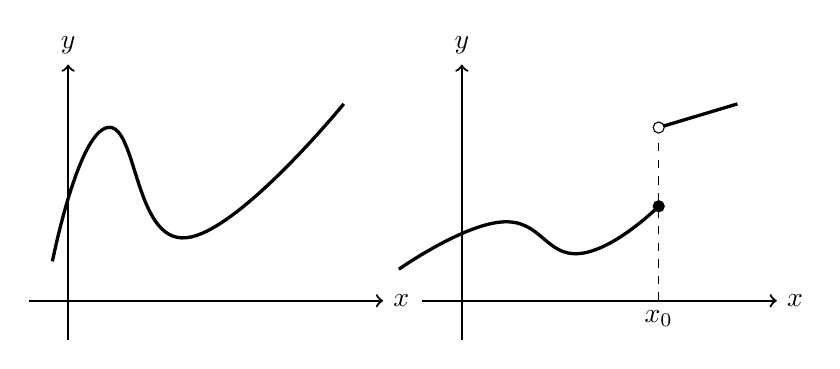
\begin{tikzpicture}
        \begin{scope}[shift={(0,0)}]
            \draw[thick, ->] (-0.5,0) -- (4,0) node[right] {$x$};
            \draw[thick, ->] (0,-0.5) -- (0,3) node[above] {$y$};
            \draw[black, very thick] plot [smooth, tension=0.8] coordinates {(-0.2,0.5) (0.5,2.2) (1.5,0.8) (3.5,2.5)};
        \end{scope}
        \begin{scope}[shift={(5,0)}]
            \draw[thick, ->] (-0.5,0) -- (4,0) node[right] {$x$};
            \draw[thick, ->] (0,-0.5) -- (0,3) node[above] {$y$};
            \draw[black, very thick] plot [smooth, tension=0.8] coordinates {(-0.8,0.4) (0.5,1) (1.5,0.6) (2.5,1.2)};
            \draw[black, very thick] plot [smooth, tension=0.8] coordinates {(2.5,2.2) (3.5,2.5)};
            \draw[dashed] (2.5,0) -- (2.5,2.1);
            \node[below] at (2.5,0) {$x_0$};
            \draw[fill=white] (2.5,2.2) circle (2pt);
            \draw[fill=black] (2.5,1.2) circle (2pt);
        \end{scope}
    
    \end{tikzpicture}
\end{center}
Analytically, we say a function $f(x)$ is continuous at $x_{0}: \text{ when } x\to x_{0} \text{ we have }f(x) \to f(x_{0})$. 

\begin{definition}{\quad Continuity of a Function at a Point}{def_4_8_1}
    Suppose a function $f(x)$ is defined in the neighborhood of $x_{0}$ and $\lim\limits_{x\to x_{0}}f(x) = f(x_{0})$, then we say that the function $f(x)$ is continuous at $x_{0}$. 
    \[
        \forall\,\epsilon>0, \,\exists\,\delta>0, \,\forall\, x, \,(\vert x-x_{0}\vert < \delta): \vert\ f(x)-f(x_{0}) \vert < \epsilon. 
    \]
\end{definition}

\begin{definition}{\quad Continuity of a Function on an Open Interval}{def_4_8_2}
    A function $ f $ is continuous on an open interval $ (a, b) $ if it is continuous at every point $ x \in (a, b) $.
\end{definition}

\begin{example}{\quad}{exp_4_8_1}
    For $f(x)=\frac{1}{x}$, show that $f(x)$ is continuous on $(0,1)$.
\end{example}

\begin{proof}{MyExpColor}
    Let $x_{0}$ be any point on the interval $(0,1)$. For all $\epsilon>0$, we need to find a $\delta>0, \,\forall\, x,\, (\vert x-x_{0} \vert<\delta): \left\vert \frac{1}{x} - \frac{1}{x_{0}}\right\vert < \epsilon$.
    \begin{align*}
        \left\vert \frac{1}{x} - \frac{1}{x_{0}}\right\vert = \left\vert \frac{x_{0}-x}{xx_{0}}\right\vert \textcolor{red}{\,< \,} \frac{2\vert x-x_{0}\vert}{\vert x_{0}\vert ^{2}}< \epsilon
    \end{align*}
    The red inequality is due to $\vert x- x_{0}\vert < \frac{x_{0}}{2} \Longleftrightarrow x > \frac{x_{0}}{2}$.
    We choose $\delta = \min\left\{\frac{x_{0}}{2},\frac{\vert x_{0}\vert^{2}\epsilon}{2}\right\}$. 
\end{proof}

\begin{definition}{\quad Left- and Right- Continuity of a Function at a Point}{def_4_8_3}
    If $\lim\limits_{x\to x_{0}^{-}}f(x) = f(x_{0})$, we say that $f(x)$ is \textbf{left-continuous} at point $x_{0}$.
    \[
        \forall\,\epsilon>0, \,\exists\, \delta >0, \,\forall\,x,\,\left( -\delta < x- x_{0} \textcolor{red}{\,\leq\,} 0 \right): \left\vert f(x)-f(x_{0})\right\vert <\epsilon
    \]
    If $\lim\limits_{x\to x_{0}^{+}}f(x) = f(x_{0})$, we say that $f(x)$ is \textbf{right-continuous} at point $x_{0}$.
    \[
        \forall\,\epsilon>0, \,\exists\, \delta >0, \,\forall\,x,\,\left( 0 \textcolor{red}{\,\leq\,} x- x_{0} < \delta \right): \left\vert f(x)-f(x_{0})\right\vert <\epsilon
    \]
\end{definition}

\begin{note}
    Note the difference in red to the left- and right-limit. 
\end{note}

\begin{definition}{\quad Continuity of a Function on an Closed Interval}{def_4_8_4}
    If a function $f(x)$ is continuous on $(a, b)$, right-continuous at point $a$, and left-continuous at point $b$, then we say that function $f(x)$ is continuous on $[a, b]$.
\end{definition}

\begin{example}{\quad}{exp_4_8_2}
    For $f(x)=\sqrt{x(1-x)}$, prove $f(x)$ is continuous on $[0,1]$. 

    [Hint:] We need to prove three things: $1.)\, f(x)$ is continuous on $(0,1)$; $2.) \, f(x)$ is right-continuous at $0$; and $3.) \, f(x)$ is left-continuous at $1$.
\end{example}

\begin{proof}{MyExpColor}
    First, let $x_{0}$ be any point in $(0,1)$. Let $\eta = \min\left\{ x_{0}, 1-x_{0}\right\}>0$. When $\left\vert x-x_{0}\right\vert < \eta$, we want to find a $\delta$ such that $\forall\, \epsilon >0, \,\forall\,x,\, (\vert x-x_{0}\vert<\delta):\vert \sqrt{x(1-x)}- \sqrt{x_{0}(1-x_{0})}\vert<\epsilon$.
    
    \begin{align*}
        \left\vert \sqrt{x(1-x)}- \sqrt{x_{0}(1-x_{0})}\right\vert = \frac{\left\vert x(1-x) - x_{0}(1-x_{0})\right\vert}{\sqrt{x(1-x)}+ \sqrt{x_{0}(1-x_{0})}} \\
        = \frac{\left\vert x-x^{2} - x_{0} + x_{0}^{2}\right\vert}{\sqrt{x(1-x)}+ \sqrt{x_{0}(1-x_{0})}} = \frac{\left\vert (x-x_{0})(1-x - x_{0})\right\vert}{\sqrt{x(1-x)}+ \sqrt{x_{0}(1-x_{0})}} \\
        = \frac{\left\vert 1-x - x_{0}\right\vert}{\sqrt{x(1-x)}+ \sqrt{x_{0}(1-x_{0})}} \left\vert (x-x_{0})\right\vert \textcolor{red}{\,<\,} \frac{1}{\sqrt{x_{0}(1-x_{0})}} \left\vert (x-x_{0})\right\vert 
    \end{align*}
    
    We choose $\delta = \min\left\{ \eta , \sqrt{x_{0}(1-x_{0})}\cdot \epsilon\right\}$, such that $\,\forall\, x,\, (\left\vert x-x_{0}\right\vert < \delta)$ we have $\left\vert \sqrt{x(1-x)}- \sqrt{x_{0}(1-x_{0})}\right\vert < \epsilon$. 

    Secondly, for $x_{0}=0$, we want to show $\lim\limits_{x\to 0+}\sqrt{x(1-x)} = 0$. For all $\epsilon >0$, we want to find a $\delta >0, \,\forall\, x,\, (0 \leq x-0 < \delta): \vert \sqrt{x(1-x) - 0}\vert < \epsilon$.
    
    \begin{align*}
        \sqrt{x(1-x)} \textcolor{red}{\,<\,} \sqrt{x} < \epsilon.
    \end{align*}
    
    We find $\delta = \epsilon^{2}, \,\forall\, x, \, (0 \leq \vert x- 0\vert <\delta): \left\vert \sqrt{1-x} - 0\right\vert < \epsilon$. 

    Thirdly, for $x_{0}=1$, we want to show $\lim\limits_{x\to 1^{-}}\sqrt{x(1-x)} = 0$. For all $\epsilon > 0$, we want to find a $\delta>0, \,\forall\, x,\, (-\delta < \vert x - 1\vert \leq 0) : \left\vert \sqrt{x(1-x)} - 0 \right\vert < \epsilon$.
    \begin{align*}
        \left\vert \sqrt{x(1-x)} \right\vert <  \sqrt{1-x} < \epsilon.
    \end{align*}
    We find $\delta = \epsilon^{2}, \,\forall\, x,\, (-\delta < x - 1 \leq 0): \left\vert\sqrt{x(1-x)} - 0 \right\vert < \epsilon$. 

    Therefore, we have shown that $f(x) = \sqrt{x(1-x)}$ is continuous on $[0,1]$.
\end{proof}

\begin{remark}
    It seems a bit tedious to show three things. A more efficient way is given below, which eliminates the need for three different definitions.
\end{remark}

\begin{definition}{\quad Continuity of a Function on Some Interval}{def_4_8_5}
    Suppose $f(x)$ is defined on some interval $X$, if $x_{0}\in X$, $\,\forall\, \epsilon>0, \,\exists\, \delta >0, \,\textcolor{red}{\forall\, x \in X}, \,\left(\left\vert x-x_{0}\right\vert < \delta \right): \left\vert f(x) - f(x_{0})\right\vert < \epsilon$, then we say $f(x)$ is continuous on the interval $X$.
\end{definition}

\begin{example}{\quad}{exp_4_8_3}
    Suppose $f(x) = \sin x$, show that $f(x)$ is continuous on $(-\infty, +\infty)$.
\end{example}

\begin{proof}{MyExpColor}
    Let $x_{0}$ be any point in $(-\infty, \infty)$, for all $\epsilon > 0$, we want to find a $\delta>0, \,\forall\, x\in (-\infty,\infty), \, \left(\left\vert x- x_{0} \right\vert < \delta\right) : \left\vert \sin x - \sin x_{0}\right\vert < \epsilon$.
    \begin{align*}
        \left\vert \sin x - \sin x_{0}\right\vert = \left\vert 2\cos\frac{x+x_{0}}{2}\sin\frac{x-x_{0}}{2} \right\vert \textcolor{blue}{\,\leq\,} 2\left\vert\sin\frac{x-x_{0}}{2} \right\vert \textcolor{red}{\,\leq\,} \left\vert x-x_{0}\right\vert < \epsilon.
    \end{align*}
    We find $\delta = \epsilon$. 

    We have shown that $f(x) = \sin x$ is continuous on $(-\infty, +\infty)$.
\end{proof}

\begin{note}
    The blue inequality is due to $\cos x \leq 1$, the red inequality is because $\lim\limits_{x\to 0}\frac{\sin x}{x} \leq 1$.
\end{note}

\begin{example}{\quad}{exp_4_8_4}
    For $f(x) = a^{x}, a> 0, a\neq 1$, show $f(x)$ is continuous on $(-\infty, +\infty)$.
\end{example}

\begin{proof}{MyExpColor}
    Let $x_{0} \in (-\infty, + \infty)$, we want to show 
    \[
        \lim\limits_{x\to x_{0}}a^{x} = a^{x_{0}} \Longleftrightarrow \lim\limits_{x\to x_{0}}a^{x-x_{0}} = 1 \Longleftrightarrow \lim\limits_{t\to 0}a^{t} = 1.
    \]
    
    For $t\to 0^{+}:$
    \begin{enumerate}
        \item [1.)] $a>1$: We note that $\frac{1}{t} \geq \left\lfloor\frac{1}{t}\right\rfloor$ and $a^{t} = ^{\frac{1}{\frac{1}{t}}} \leq a^{\frac{1}{\left\lfloor\frac{1}{t} \right\rfloor}}$. Also, $\frac{1}{t} \xrightarrow{t\to 0}+\infty$, view \textcolor{blue}{$\left\lfloor \frac{1}{t} \right\rfloor$} as \textcolor{blue}{$n$}, and recall that we have shown $\lim\limits_{n\to+\infty}\sqrt[n]{a} = \lim\limits_{n\to+\infty} a^{\frac{1}{n}} = 1$. We have 
        \[
            1 < a^{t} \leq a^{\frac{1}{\left\lfloor\frac{1}{t}\right\rfloor}}.
        \]
        Thus, by the Squeeze theorem, we have $\lim\limits_{t\to 0}a^{t} = 1$.
        \item [2.)] $0<a<1$: We have $\lim\limits_{t\to 0^{+}}a^{t} = \lim\limits_{t\to 0+}\frac{1}{\left(\frac{1}{a}\right)^{t}} = 1$.
    \end{enumerate}

    For $t \to 0^{-}:$ 
    \begin{enumerate}
        \item[] Let $u=-t$, then $u \to 0^{+}$. Then
    \end{enumerate}
         \[
            \lim\limits_{t\to 0^{-}}a^{t} = \lim\limits_{u\to 0^{+}}a^{-u} = \lim\limits_{u\to 0^{+}}\frac{1}{a^{u}} = 1.
         \]
    Since $\lim\limits_{t\to 0^{-}}a^{t} = \lim\limits_{t\to 0^{+}}a^{t}$, we have shown $\lim\limits_{t\to 0}a^{t} = \lim\limits_{x\to x_{0}}a^{x} = 1$.
\end{proof}



\section{The Arithmetic Operations on Limits of The Continuous Functions}
\begin{theorem}{\quad}{thm_4_9_1}
    Suppose $f(x)$ and $g(x)$ are two continuous functions at the point $x_{0}$. That is $\lim\limits_{x\to x_{0}}f(x) =f(x_{0})$ and $\lim\limits_{x\to x_{0}}g(x) = g(x_{0})$.
    
    \begin{enumerate}[topsep=10pt, itemsep=5pt]
        \item $\lim\limits_{x\to x_{0}}\left(\alpha f(x) + \beta g(x)\right) = \alpha f(x_{0}) + \beta g(x_{0})$;
        \item $\quad \lim\limits_{x\to x_{0}}\left(f(x)g(x)\right) = f(x_{0})g(x_{0})$; 
        \item $\quad \lim\limits_{x\to x_{0}}\frac{f(x)}{g(x)} = \frac{f(x_{0})}{g(x_{0})}, \quad g(x_{0}) \neq 0$.
    \end{enumerate}
\end{theorem}

\begin{example}{\quad}{exp_4_9_1}
    Find the value of $\lim\limits_{x\to2}\frac{x^{2} + \sin x}{3^{x} + 2x}$.
\end{example}

\begin{solve}{MyExpColor}
    It is obvious that the answer is $\frac{4 + \sin 2}{13}$, since all four functions are continuous at $x=2$.
\end{solve}

\begin{example}{\quad}{exp_4_9_2}
    The polynomial $P_{n}(x) = a_{n}x^{n} + a_{n-1}x^{n-1} + \,\dots\, + a_{0}$ is continuous on $(-\infty, +\infty)$.
    
    The polynomial $Q_{m}(x) = \frac{P_{n}(x)}{b_{m}x^{m} + b_{m-1}x^{m-1} + \,\dots\, + b_{0}}$ is continuous on its domain.
\end{example}

\begin{example}{\quad}{exp_4_9_3}
    We know that $\sin x$ and $\cos x$ are continuous on $(-\infty, +\infty)$, then it is obvious that

    \begin{enumerate}[topsep=10pt, itemsep=5pt]
        \item [1.)] $\tan x = \frac{\sin x}{\cos x}$ is continuous on $\left\{ x \mid x\neq k\pi +\frac{\pi}{2}, k \in\mathbb{Z}\right\}$;
        \item [2.)] $\cot x = \frac{\cos x}{\sin x}$ is continuous on $\left\{ x \mid x\neq k\pi, k \in\mathbb{Z}\right\}$.
    \end{enumerate}
\end{example}



\section{Types of Discontinuities}
Before we discuss different types of discontinuities, let's have a closer look at $\lim\limits_{x\to x_{0}}f(x) = f(x_{0})$. What does it mean by saying $\lim\limits_{x\to x_{0}}f(x) = f(x_{0})$?

\begin{enumerate}[topsep=10pt, itemsep=5pt]
    \item $f(x)$ is defined at $x_{0}$;
    \item $\lim\limits_{x\to x_{0}^{+}}f(x) = f(x_{0})$;
    \item $\lim\limits_{x\to x_{0}^{-}}f(x) = f(x_{0})$. 
\end{enumerate}
Missing any one of these three conditions at the point $x_{0}$, $f(x)$ is considered discontinuous at $x_{0}$.

\begin{definition}{\quad Types of Discontinuities}{def_4_10_1}
    There are four types of discontinuities:

    \begin{enumerate}[topsep=10pt, itemsep=5pt]
        \item \textbf{Jump Discontinuity}: $\lim\limits_{x\to x_{0}^{+}}f(x) \neq \lim\limits_{x\to x_{0}^{-}}f(x)$;
        \item \textbf{Oscillatory Discontinuity}: As $x$ approaches $x_{0}$, the function $f(x)$ fluctuates between different values (e.g., between $-1$ and $1$) with increasing frequency, preventing the limit from settling on a single value.
        \item \textbf{Infinite Discontinuity}: At least one of the $\lim\limits_{x\to x_{0}^{+}}f(x)$ and $\lim\limits_{x\to x_{0}^{-}}f(x)$ does not converge;
        \item \textbf{Removable Discontinuity}: Removable discontinuity occurs at a point $x_{0}$ in the domain of a function $ f(x) $ when the function is not defined at $ x_{0} $ or the value of the function at $ x_{0} $ does not match the limit, but the limit $ \lim_{x \to x_{0}} f(x) $ exists and is finite. This means the discontinuity can be "removed" by redefining the function at $ x_{0} $ to equal the limit, making the function continuous at that point. That is
        \[
            \lim\limits_{x\to x_{0}^{+}}f(x) = \lim\limits_{x\to x_{0}^{-}}f(x) \begin{cases}
                \neq f(x_{0}), \\
                \text{or }f(x) \text{ is not defined at } x_{0}.
            \end{cases}
        \]
    \end{enumerate}
\end{definition}

\begin{example}{\quad Dirichlet Function}{exp_4_10_1}
Prove that the Dirichlet function, $D(x)$, is not continuous on $(-\infty, + \infty)$.
    \[
        D(x) = \begin{cases}
            1\quad \text{if } x \in \mathbb{Q}, \\
            0\quad \text{if } x \notin \mathbb{Q}.
        \end{cases}
    \]

    \begin{center}
        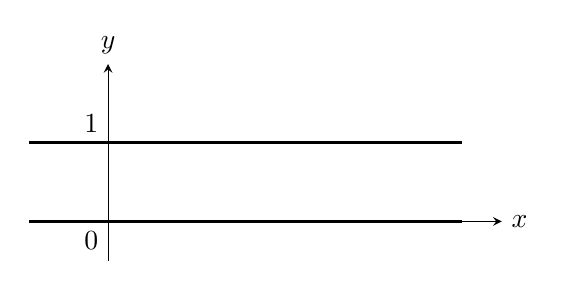
\begin{tikzpicture}[>=stealth]
            \draw[->] (-1,0) -- (5,0) node[right] {$x$};
            \draw[->] (0,-0.5) -- (0,2) node[above] {$y$};
            \draw[very thick] (-1,1) -- (4.5,1);
            \draw[very thick] (-1,0) -- (4.5,0);
            \node[below left] at (0,0) {$0$};
            \node[above left] at (0,1) {$1$};
        \end{tikzpicture}
    \end{center}
\end{example}

\begin{proof}{MyExpColor}
    Let $x_{0} \in (-\infty, +\infty)$. Let $x_{n}^{\prime}$ be any rational, $x_{n}^{\prime} > x_{0}, x_{n}^{\prime} \to x_{0}$, then 
    \[
        \lim\limits_{x_{n}^{\prime}\to x_{0}}D(x_{n}^{\prime}) = 1.
    \]
    Let $x_{n}^{\prime\prime}$ be any irrational, $x_{n}^{\prime\prime} > x_{0}, x_{n}^{\prime\prime} \to x_{0}$, then 
    \[
        \lim\limits_{x_{n}^{\prime\prime}\to x_{0}}D(x_{n}^{\prime\prime}) = 0.
    \]
By Heine theorem, we know that $\lim\limits_{x\to x_{0}}D(x)$ does not exists. Since $x_{0} \in (-\infty, +\infty)$, we know that the Dirichlet Function, $D(x)$, is not continuous on $(-\infty, + \infty)$.
\end{proof}

\begin{example}{Popcorn Function}{exp_4_10_2}
Prove for all $x_{0} \in (-\infty, +\infty)$, $\lim\limits_{x\to x_{0}}R(x) = 0$. That is the Popcorn function is continuous at all irrationals and it is discontinuous at all rationals.
    \[
        R(x) = \begin{cases}
            0 \quad \text{if } x \notin \mathbb{Q}, \\
            \frac{1}{p} \quad \text{if } p \in \mathbb{N}^{+}, q \in \mathbb{Z}\backslash\{0\}, p \text{ and } q \text{ co-prime}, \\
            1 \quad \text{if } x = 0.
        \end{cases}
    \]
    \begin{center}
        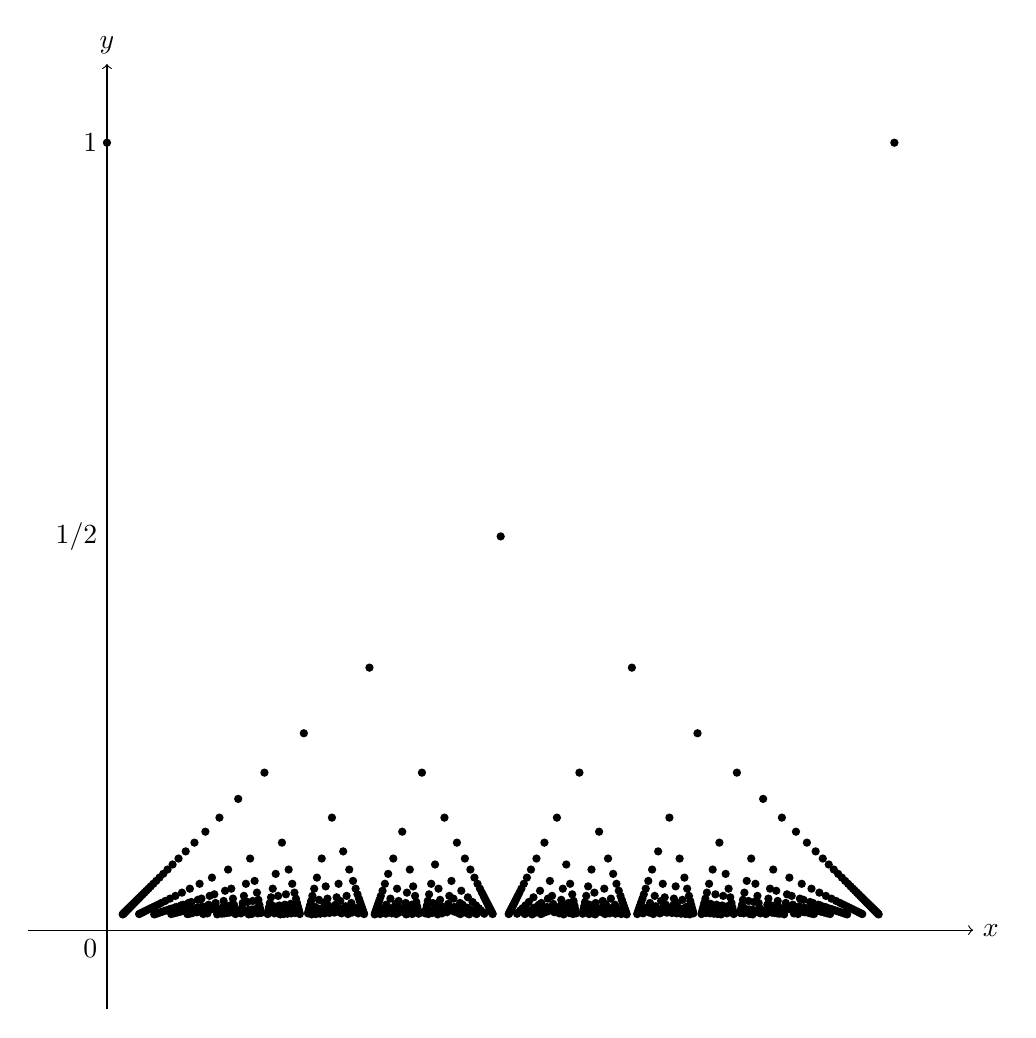
\begin{tikzpicture}[scale=10]
            \draw[->] (-0.1,0) -- (1.1,0) node[right] {$x$};
            \draw[->] (0,-0.1) -- (0,1.1) node[above] {$y$};
            \def\maxden{50}
            \foreach \q in {1,...,\maxden} {
                \foreach \p in {0,...,\q} {
                    \pgfmathsetmacro{\g}{gcd(\p,\q)}
                    \ifnum\g=1
                        \fill (\p/\q, 1/\q) circle (0.15pt);
                    \fi
                }
            }
            \node[left] at (0,1) {$1$};
            \node[left] at (0,0.5) {$1/2$};
            \node[below left] at (0,0) {$0$};
        \end{tikzpicture}
    \end{center}
    Here, $x=0, R(x) = 1$ is to maintain the periodicity of the Popcorn function.
\end{example}

\begin{proof}{MyExpColor}
    Consider the periodicity, we only need to consider $x_{0} \in [0,1]$. That is we only need to show for $x_{0} \in [0,1], \lim\limits_{x\to x_{0}}R(x) = 0$\dots
    \begin{enumerate}[topsep=10pt, itemsep=5pt]
        \item In $[0,1]$, the number of numbers that have $1$ as their denominator is $2$: $\quad \frac{0}{1}, \frac{1}{1}$
        \item In $[0,1]$, the number of numbers that have $2$ as their denominator is $1$: $\quad \frac{1}{2}$;
        \item In $[0,1]$, the number of numbers that have $3$ as their denominator is $2$: $\quad \frac{1}{3}, \frac{2}{3}$;
        \item $\dots \dots$ 
        \item In $[0,1]$, the number of numbers that have $k$ as their denominator is: at most $k$.
    \end{enumerate}

    For any $k \in \mathbb{Z}^{+}$, there are finitely many rational numbers on $[0,1]$ with denominators \uwave{less than or equal to $k$}. 

    \uwave{For all $\epsilon > 0$}, find $\delta > 0$. Let $k = \left\lfloor\frac{1}{\epsilon}\right\rfloor$. In $[0,1]$, denote the rationals whose denominator is less than or equal to $k$ as $r_{1}, r_{2}, \dots, r_{n}$. Let \uwave{$\delta = \min\limits_{\substack{1 \leq i \leq n \\ r_{i} \neq x_{0}}} \left\{\left\vert r_{i} - x_{0} \right\vert\right\}$}, $\forall\, x\in [0,1],\, \left(0 < \left\vert x-x_{0}\right\vert< \delta\right)$. 

    \begin{enumerate}[topsep=10pt, itemsep=5pt]
        \item $x$ is irrational, $R(x) = 0$;
        \item [2.)] $x$ is rational, the denominator of $x$ has to be greater than $k$. Since $k = \left\lfloor\frac{1}{\epsilon}\right\rfloor$, that means the denominator is greater than or equal to $\left\lfloor\frac{1}{\epsilon}\right\rfloor + 1$.
        \[
            R(x) - 0 = \frac{1}{k} \leq \frac{1}{\left\lfloor\frac{1}{\epsilon}\right\rfloor + 1} < \frac{1}{\frac{1}{\epsilon}} = \epsilon.
        \]
    \end{enumerate}
\end{proof}


\begin{remark}
    The key difference between the Dirichlet function and Popcorn function is that the Popcorn function has the following property:
    \[
        \forall\, \epsilon > 0, \text{ there are at most limited number of points that makes } R(x) > \epsilon, \text{ on the interval } [0,1].
    \]
\end{remark}

\begin{example}{\quad}{exp_4_10_3}
    The discontinuities of a monotonic function on an interval $(a, b)$ must be the Jump discontinuity.
\end{example}

\begin{proof}{MyExpColor}
    W.O.L.G., let $f(x)$ be monotonically increasing on $(a, b)$. Let $x_{0}\in (a,b)$. The set $\left\{f(x) \mid x\in(a, x_{0}) \right\}$ has a upper bound and must have a supremum, denoted $\alpha = \sup\left\{ f(x) \mid x\in (a,x_{0})\right\}$. For all $x\in(a, x_{0})$ we have $f(x) \leq \alpha$. That is \uwave{$\,\forall\, \epsilon > 0$},$ \,\exists\, x^{\prime} \in (a, x_{0})$ such that $f(x^{\prime}) > \alpha - \epsilon$. Let \uwave{$\delta = x_{0} - x^{\prime}$}, \uwave{$\,\forall\, x, \, \left( -\delta < x-x_{0} < 0 \right)$}. That is saying $x \in (x^{\prime}, x_{0})$. Since $f(x)$ is monotonically increasing, we have 
    \begin{center}
        \begin{tikzpicture}[>=stealth, scale=1.5]
            \draw[thick, ->] (-0.5,0) -- (6.5,0);
            \node at (0,0) {\textbf{(}};
            \node[below=4pt] at (0,0) {$a$};
            \filldraw (2,0) circle (1pt) node[below=4pt] {$x'$};
            \draw[<-] (3.2,0.1) -- (3.6,0.6) node[above] {$x$};
            \node at (4,0) {\textbf{)}};
            \node[below=4pt] at (4,0) {$x_0$};
            \node at (6,0) {\textbf{)}};
            \node[below=4pt] at (6,0) {$b$};
        \end{tikzpicture}
    \end{center}
    
    \[
        \alpha -\epsilon < f(x^{\prime}) \leq f(x) \leq \alpha
    \]
    
    Therefore, we have $\left\vert f(x) - \alpha\right\vert < \epsilon$, that is $ \lim\limits_{x\to x_{0}^{-}}f(x) = \alpha.$

    Similarly, 
    
    \[
        \lim\limits_{x\to x_{0}^{+}}f(x) = \beta, \beta = \inf \left\{f(x) \mid x \in (x_{0}, b)\right\}
    \].
\end{proof}



\section{Inverse Function}
We will discuss two properties of the inverse function: the \textit{existence} and \textit{continuity}. We will differ the third property, \textit{differentiability}, to later sections. 

\begin{theorem}{\quad Inverse of a Monotone (or Monotonic) Function Theorem}{4.11.1}
    If a function $f(x)$ is  \uwave{strictly} monotonic (increasing or decreasing) over $D_{f}$, then there exists an inverse function $x = f^{-1}(y), y \in R_{f}$ and the inverse function $f^{-1}$ is also \uwave{strictly} monotonic (increasing or decreasing).
\end{theorem}

\begin{proof}{MyThmColor}
    For $x_{1},x_{2} \in D_{f}$ with $x_{1} < x_{2}$, it is obvious that $f(x_{1}) < f(x_{2})$ or $y_{1} < y_{2}$. Moreover, $x_{1}$ and $x_{2}$ can swap, meaning we choose them randomly. In other words, for $x_{1},x_{2} \in D_{f}$ with $x_{1} > x_{2}$, it is obvious that $f(x_{1}) > f(x_{2})$ or $y_{1} > y_{2}$. Then it is easy to see that if $x_{1} \neq x_{2}$ then $y_{1} \neq y_{2}$ (Injection). Therefore, there exists an inverse function $x = f^{-1}(y)$. Now $\forall\, y_{1} < y_{2}$, if $x_{1} > x_{2}$ is a contradiction to \uwave{strictly} monotonic increasing for the function $f(x)$. If $x_{1} = x_{2}$, this is a contradiction to the definition of a function. So $x_{1} < x_{2}$ that is $f^{-1}(y)$ is \uwave{strictly} monotonic increasing.
\end{proof}

\begin{note}
    In short: If $f$ is strictly monotonic, then $f^{-1}$ exists and is also strictly monotonic. This takes care of the \textit{existence}.
\end{note}

\begin{theorem}{\quad Continuity of the Inverse Function Theorem for Monotonic Functions}{thm_4_11_2}
    Suppose $y = f(x)$ is continuous and strictly increasing on the interval $[a, b]$. If $f(a) = \alpha, f(b) = \beta$, then $f^{-1}(y)$ is continuous on $[\alpha, \beta]$.
\end{theorem}

\begin{proof}{MyThmColor}
    [Hint:] First, we need to show $R_{f} = [\alpha, \beta]$. Since $f(a), f(b)$ have to be in $R_{f}$ we only need to find a point say $\gamma \in [\alpha,\beta]$ and a point $x_{0} \in [a,b]$ such that $f(x_{0}) = \gamma$, then we are done. For continuity, we need to show $f^{-1}$ is continuous at $y_{0}\in (\alpha, \beta)$ and left- and right-continuous at $\beta$ and $\alpha$.

    First, we need to show $R_{f} = [\alpha, \beta]$. Now, $\forall\, \gamma \in [\alpha, \beta]$, let $S = \left\{x \mid x\in [a,b], f(x) < \gamma\right\}$. Let $\sup S = x_{0}$. (We know $S$ has the supremum because $S$ has an upper bound.) When $x < x_{0}$, we have $f(x) < \gamma$ and when $x > x_{0}$, we have $f(x) > \gamma$, by $f$ is strictly increasing. $\lim\limits_{x\to x_{0}^{-}}f(x) \leq \gamma, \lim\limits_{x\to x_{0}^{+}}f(x) \geq \gamma$. Also, $f$ is continuous in $[a,b]$ so $f$ is continuous at $x_{0}$, therefore $\lim\limits_{x\to x_{0}^{-}}f(x) = \lim\limits_{x\to x_{0}^{+}}f(x) = f(x_{0})$. Therefore, $f(x_{0}) = \gamma$. Thus, $R_{f} = [\alpha, \beta]$. 

    Now, we deal with the continuity. For all $y_{0} \in (\alpha, \beta)$, we need to show that $f^{-1}$ is continuous at $y_{0}$ and is left- and right- continuous at $\beta$ and $\alpha$. 
    
    \begin{center}
        \begin{tikzpicture}[>=stealth, scale=1.5]
            \draw[->] (-0.5,0) -- (5,0) node[right] {$x$};
            \draw[->] (0,-0.5) -- (0,5) node[above] {$y$};
            \draw[blue, thick] (0.5,0.5) .. controls (2,1) and (3,4) .. (4.5,4.5) 
                node[pos=0.25] (p1) {} % Save position for x0 - epsilon
                node[pos=0.5]  (p0) {} % Save position for x0
                node[pos=0.75] (p2) {}; % Save position for x0 + epsilon
            \draw[dashed] (p0) -- (p0 |- 0,0) node[below] {$x_0$};
            \draw[dashed] (p0) -- (p0 -| 0,0) node[left] {$y_0$};
            \fill (p0) circle (1.5pt);
            \draw[dashed] (p1) -- (p1 |- 0,0) node[below] {$x_0 - \varepsilon$};
            \draw[dashed] (p1) -- (p1 -| 0,0) node[left] {$y_1$};
            \fill (p1) circle (1.5pt);
            \draw[dashed] (p2) -- (p2 |- 0,0) node[below] {$x_0 + \varepsilon$};
            \draw[dashed] (p2) -- (p2 -| 0,0) node[left] {$y_2$};
            \fill (p2) circle (1.5pt);
        \end{tikzpicture}
    \end{center}
    
    Here, we only prove one of them. Let $f(x_{0}) = y_{0}$ that is $f^{-1}(y_{0}) = x_{0}$. We need to show that $\forall\, \epsilon > 0,$ we need to find $\delta > 0, \forall\, y,\, \left(\vert y-y_{0}\vert < \delta\right): \underbrace{\left\vert f^{-1}(y)-f^{-1}(y_{0})\right\vert < \epsilon}_{\vert x-x_{0}\vert \,<\, \epsilon}$. Let $\delta = \min \left\{y_{0} - y_{1}, y_{2}-y_{0} \right\}$, when $\vert y-y_{0}\vert < \delta$, there is $\vert x-x_{0}\vert < \epsilon$. The left- and right-continuity at $\beta$ and $\alpha$ are left as exercises.
\end{proof}

\begin{example}{\quad}{exp_4_11_1}
    For $y=\sin x$, which is continuous and strictly increasing on it domain $\left[-\frac{\pi}{2}, \frac{\pi}{2}\right]$ and its range is $[-1,1]$. Its inverse function $y = \sin^{-1}x= \arcsin x$ has domain $D=[-1, 1]$ (continuous and strictly increasing over $[-1, 1]$) and range $R = \left[-\frac{\pi}{2}, \frac{\pi}{2}\right]$.

    \begin{center}
        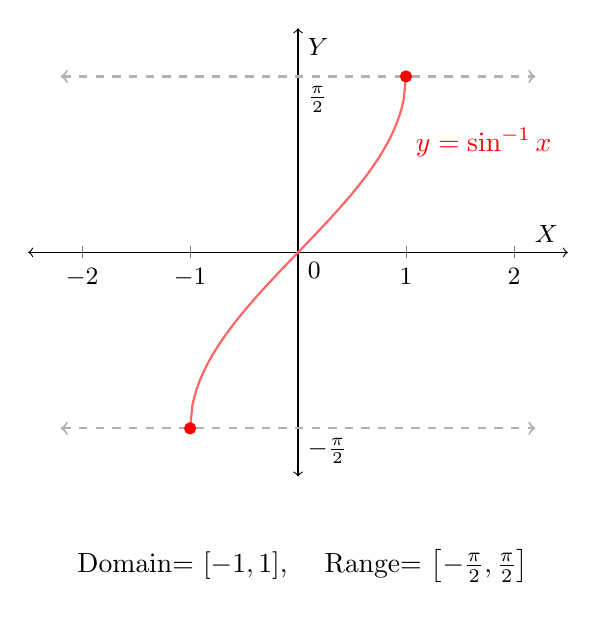
\begin{tikzpicture}
            \begin{axis}[
                axis lines = middle,
                xlabel = {$X$},
                ylabel = {$Y$},
                xmin = -2.5, xmax = 2.5,
                ymin = -2, ymax = 2,
                xtick = {-2, -1, 1, 2}, % Removed 0 to handle it manually
                ytick = \empty,          
                axis line style={<->},
                label style={font=\small},
                tick label style={font=\small},
            ]
                \draw[dashed, gray!60, thick, <->] (axis cs:-2.2, 1.57) -- (axis cs:2.2, 1.57);
                \draw[dashed, gray!60, thick, <->] (axis cs:-2.2, -1.57) -- (axis cs:2.2, -1.57);
                \node[anchor=north west, font=\small] at (axis cs:0, 1.57) {$\frac{\pi}{2}$};
                \node[anchor=north west, font=\small] at (axis cs:0, 0) {$0$};
                \node[anchor=north west, font=\small] at (axis cs:0, -1.57) {$-\frac{\pi}{2}$};
                \addplot [
                    domain=-1:1, 
                    samples=100, 
                    color=red!60, 
                    thick,
                ] {asin(x)*pi/180}; 
                \addplot[only marks, mark=*, color=red] coordinates {(-1, -1.57) (1, 1.57)};
                \node[anchor=north west, color=red] at (axis cs:1.0, 1.2) {$y = \sin^{-1} x$};
            \end{axis}
            \node[anchor=north west, align=left] at (0.5,-0.8) {
                Domain= $[-1, 1]$, \quad Range= $\left[-\frac{\pi}{2}, \frac{\pi}{2}\right]$
            };
        \end{tikzpicture}
    \end{center}
\end{example}

Now, let us talk about the composite function. If we compose two continuous functions together, is it still continuous.

\begin{example}{\quad}{exp_4_11_2}
    If $\lim\limits_{u\to u_{0}}f(u) = A, \lim\limits_{x\to x_{0}}g(x) = u_{0}$, does $\lim\limits_{x\to x_{0}}f\circ g(x)= A$ hold?
\end{example}

\begin{solve}{MyExpColor}
    The answer is No! A counter example would be
    
    \[
    f(u) = 
    \begin{cases}
        0 \quad \text{if } u=0, \\
        1 \quad \text{if } u\neq 0.
    \end{cases}
    g(x) = x\sin \frac{1}{x}
    \]
    
    \begin{center}
        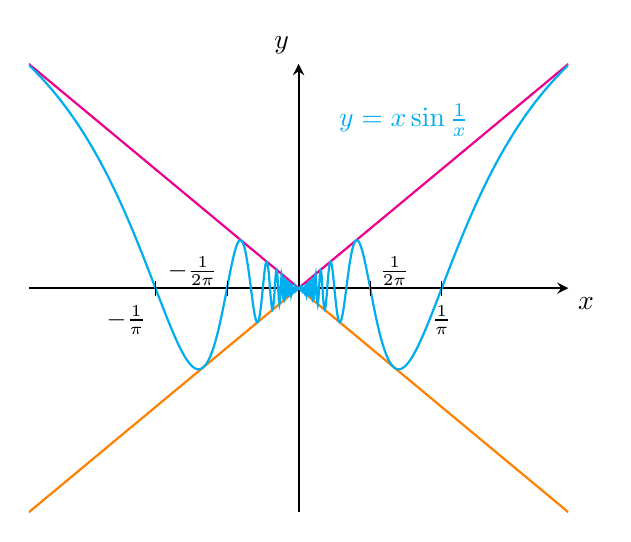
\begin{tikzpicture}
            \begin{axis}[
                axis lines = middle,
                xlabel = {$x$},
                ylabel = {$y$},
                xmin = -0.6, xmax = 0.6,
                ymin = -0.6, ymax = 0.6,
                ticks = none,
                axis line style={thick, black, -stealth},
                xlabel style={black, anchor=north west},
                ylabel style={black, anchor=south east},
            ]
                \addplot [domain=-0.6:0.6, samples=3, magenta, thick] {abs(x)}; % y = |x|
                \addplot [domain=-0.6:0.6, samples=3, orange, thick] {-abs(x)}; % y = -|x|
                \addplot [
                    domain=-0.6:0.6, 
                    samples=1000, 
                    cyan, 
                    thick,
                    restrict y to domain=-1:1,
                ] {x * sin(deg(1/x))}; 
                \draw[black] (axis cs:0.318, 0.02) -- (axis cs:0.318, -0.02) node[below] {\small $\frac{1}{\pi}$};
                \draw[black] (axis cs:0.159, 0.02) -- (axis cs:0.159, -0.02) node[above right] {\small $\frac{1}{2\pi}$};
                \draw[black] (axis cs:-0.318, 0.02) -- (axis cs:-0.318, -0.02) node[below left] {\small $-\frac{1}{\pi}$};
                \draw[black] (axis cs:-0.159, 0.02) -- (axis cs:-0.159, -0.02) node[above left] {\small $-\frac{1}{2\pi}$};
                \node[cyan, anchor=east] at (axis cs:0.4, 0.45) {$y = x \sin \frac{1}{x}$};
            \end{axis}
        \end{tikzpicture}
    \end{center}
    
    It is obvious that $\lim\limits_{u\to0}f(u)=1$ and $\lim\limits_{x\to0}g(x)=0$. Then we have 
    
    \[
    f\circ g(x) = 
    \begin{cases}
        0 \quad \text{if } x = \frac{1}{n\pi},\\
        1 \quad \text{if } x \neq \frac{1}{n\pi}.
    \end{cases}
    \]
    
    Now, we want to use the Heine Theorem \ref{:thm_4_4_1}. We need to find two sequences that five two different limits for $f\circ g(x)$.
    Let the first sequence be $\left\{x_{n}^{\prime}\right\}, x_{n}^{\prime} = \frac{1}{n\pi}$, it is obvious that $x_{n}^{\prime} \xrightarrow[]{n\to +\infty} 0$, and $\lim\limits_{n\to+\infty}f\circ g(x_{n}^{\prime}) = 0$. Let the second sequence be $\left\{x_{n}^{\prime\prime}\right\}, x_{n}^{\prime\prime} \neq \frac{1}{k\pi}$, it is obvious that $x_{n}^{\prime\prime} \xrightarrow[]{n\to+\infty}0$, but $\lim\limits_{n\to+\infty}f\circ g(x_{n}^{\prime\prime}) = 1$. So we find two difference sequences that are not zero, but approaches zero give two difference limits to $f\circ g(x)$. Therefore, we know that $\lim\limits_{x\to 0}f\circ g(x)$ does not exist.
\end{solve}

\begin{note}
    In example \ref{:exp_4_11_2}, it is because $f(u)$ is  discontinuous at $u=0$ that makes the statement in example \ref{:exp_4_11_2} invalid.
\end{note}

\begin{theorem}{\quad}{thm_4_11_3}
    If $u=g(x)$ is continuous at $x_{0}$ that is $\lim\limits_{x\to x_{0}}g(x) = u_{0}$, and $g(x_{0})=u_{0}$. Also, if $f(u)$ is continuous at $u_{0}$ that is $\lim\limits_{u\to u_{0}}f(u) = f(u_{0})$, then $f\circ g$ is continuous at $x_{0}$ that is $\lim\limits_{x\to x_{0}}f\circ g(x) = f\circ g(x_{0}) = f(u_{0})$.
\end{theorem}

\begin{proof}{MyThmColor}
    \uwave{For all $\epsilon > 0$}, $\,\exists\, \eta > 0, \,\forall\, u, \, (\vert u-u_{0} \vert < \eta): \vert f(u) - f(u_{0})\vert < \epsilon $. For all $\eta >0$, \uwave{$\,\exists \delta > 0, \,\forall\, x, \, (\vert x-x_{0}\vert < \delta)$}$:\vert g(x) - g(x_{0})\vert < \eta$. That is $\left\vert g(x) - u_{0}\right\vert < \eta$. That is \uwave{$\left\vert f\circ g(x) - f\circ g(x_{0}) \right\vert < \epsilon$}.
\end{proof}

\begin{note}
    For $f\circ g$ to be a continuous, functions $f$ and $g$ both have to be continuous. Also, do not forget that the range of $g$ has to sit within the domain of $f$.    
\end{note}

\begin{example}{\quad}{exp_4_11_3}
Given $y = \sinh x = \frac{e^{x} - e^{-x}}{2}$ and $\cosh x = \frac{e^{x} + e^{-x}}{2}$. Let $u=e^{x}$, then $y=\frac{u-u^{-1}}{2}$. Applying the theorem above we know that $\sinh x$ is continuous. It is similar to show $\cosh x$ is continuous.
\end{example}

\begin{example}{\quad}{exp_4_11_4}
    Prove for any real number $\alpha$, $f(x) = x^{\alpha}$ is continuous on $(0, +\infty)$.
\end{example}
\begin{proof}{MyExpColor}
    W.O.L.G., $f(x) = x^{\alpha}=e^{\alpha \ln x}$. That is $y=e^{u}$ and $u=\alpha \ln x$. First, the range of $u$, which is $R_{u} = (0, +\infty)$, is in the domain of $y$, which is $D_{y} = (-\infty, +\infty)$. Both $u$ and $y$ are continuous in their domain, so their composite $f(x) = y\circ u(x)$ is continuous by applying theorem \ref{:thm_4_11_3}.
\end{proof}
\begin{note}
    Several things to point out:

    \begin{enumerate}[topsep=10pt, itemsep=5pt]
        \item When $\alpha = n, n \in \mathbb{Z}^{+}$, $f(x)=x^{n}$ is continuous on $(-\infty, +\infty)$.
        \item When $\alpha = -n, n \in \mathbb{Z}^{+}$, $f(x) = x^{-n}$ is continuous on $(-\infty, 0) \cup (0, +\infty)$.
        \item When $\alpha = \frac{q}{p}, p, q$ are co-primes, 
        \begin{enumerate}[topsep=10pt, itemsep=5pt]
            \item if $p$ is odd, $f(x) = x^{\frac{q}{p}}$ is continuous on $(-\infty, +\infty)$.
            \item if $p$ is even $f(x) = x^{\frac{q}{p}}$ is continuous on $[0, +\infty)$.
        \end{enumerate}
    \end{enumerate}
\end{note}

\begin{definition}{\quad Basic Elementary Functions}{def_4_11_1}
    \textbf{Basic elementary functions} are functions obtained from constants, powers, exponentials, logarithms, trigonometric, and inverse trigonometric functions.
\end{definition}

\begin{definition}{\quad Elementary Functions}{def_4_11_2}
    \textbf{Elementary functions} are the functions obtained from \textbf{basic elementary functions}, using a \textit{finite} number of operations of addition, subtraction, multiplication, division, and composition.
\end{definition}

\begin{theorem}{\quad}{thm_4_11_4}
    All \textbf{elementary functions} are continuous on their domains. 
\end{theorem}

\begin{note}
    Theorem \ref{:thm_4_11_4} can help us find limit of certain types of functions.
\end{note}

\begin{example}{\quad}{exp_4_11_5}
    Compute $\lim\limits_{x\to0}\left(\cos x\right)^{\frac{1}{x^{2}}}$.
\end{example}

\begin{solve}{MyExpColor}
[Hint:] By theorem \ref{:thm_4_11_4}, we know $\left(\cos x\right)^{\frac{1}{x^{2}}}$ is continuous on its domain, which means that we only need to plugin $x=0$ into the function to find the answer. So, when $x=0$, $\cos x = 1$ then you may think the answer is $1$. Sadly, it is wrong. The limit has the \textbf{indeterminate form},  $1^{\infty}$. So, we need to work more to work this out. 

Recall, this is very similar to $\lim\limits_{n \to \infty}\left(1+\frac{1}{n}\right)^{n} = e \neq 1$. Because $1^{\infty}$ is an \textbf{indeterminate form} of limit.

We have:
    \begin{align*}
        \lim\limits_{x\to0}\left(\cos x\right)^{\frac{1}{x^{2}}} = \lim\limits_{x\to0}\left(1-2\sin^{2}\frac{x}{2}\right)^{\frac{1}{x^{2}}}
    \end{align*}
Also,
\begin{align*}
    \left(\cos x\right)^{\frac{1}{x^{2}}} = \exp \left\{\ln (\cos x)^{\frac{1}{x^{2}}}\right\} = \exp\left\{\frac{1}{x^{2}}\ln (\cos x)\right\}
\end{align*}
Combining them together, we have 
\begin{align*}
    \left(\cos x\right)^{\frac{1}{x^{2}}} = \exp\left\{\frac{1}{x^{2}}\ln \left(\cos x\right)\right\} = \exp\left\{\textcolor{blue}{\frac{1}{x^{2}}\ln \left(1-2\sin^{2}\frac{x}{2}\right)}\right\} = 
\end{align*}
Let's focus on the blue part, $\frac{1}{x^{2}}\ln \left(1-2\sin^{2}\frac{x}{2}\right) = \textcolor{ForestGreen}{\frac{2\sin^{2}\frac{x}{2}}{x^{2}}}\ln \textcolor{orange}{\left(1-2\sin^{2}\frac{x}{2}\right)^{\frac{1}{2\sin^{2}\frac{x}{2}}}}$. Also, we know
\begin{align*}
    \lim\limits_{x\to0}(1-x)^{\frac{1}{x}} &= \frac{1}{e}, \quad\quad\quad
    \lim\limits_{x\to0} \textcolor{orange}{\left(1-2\sin^{2}\frac{x}{2}\right)^{\frac{1}{2\sin^{2}\frac{x}{2}}} = \frac{1}{e}} \\
    \lim\limits_{x\to0}\textcolor{ForestGreen}{\frac{2\sin^{2}\frac{x}{2}}{x^{2}}} &= \lim\limits_{x\to0}\frac{2\sin^{2}\frac{x}{2}}{4\cdot\left( \frac{x}{2}\right)^{2}} = \frac{1}{2}
\end{align*}
Putting everything together, we have 
\begin{align*}
    \lim\limits_{x\to0}\frac{1}{x^{2}}\ln\left(1-2\sin^{2}\frac{x}{2}\right) &= -\frac{1}{2} \\
    \lim\limits_{x\to0} \frac{1}{x^{2}}\ln \cos x &= -\frac{1}{2} \\
    \lim\limits_{x\to0}\ln \,\left(\cos x\right)^{\frac{1}{x^{2}}} &= -\frac{1}{2} \\
    \lim\limits_{x\to0} \left(\cos x\right)^{\frac{1}{x^{2}}} &= e^{-\frac{1}{2}} = \frac{1}{\sqrt{e}}.
\end{align*}
\end{solve}
\begin{note}
    The big takeaway here is that when we calculating the limit of a continuous function by plugin the limit of $x$ directly, if the answer we got is indeterminate form, we know we have more work to do.
\end{note}

\begin{example}{}{exp_4_11_6}
    The mass variation of a radioactive substance. At time $t=0$, the initial total mass of the substance is $M=M(0)$, and the decay constant is $k$. Find the mass of the substance $M(t)$ at time $t$.
\end{example}

\begin{solve}{MyExpColor}
    [Hint]: The key idea is to divide time into very small intervals so that the decay differs little in each small time interval.

      We divide $(o, t]$ into $n$ small intervals $\Delta_{i} = \left(\frac{(i-1)t}{n}, \frac{it}{n}\right], i = 1, 2, \dots, n$. That is $(0,t] = \bigcup\limits_{i=1}^{n}\Delta_{i}$. Then we have 
      \begin{align*}
          \Delta_{1}: \quad M\left(\frac{t}{n}\right) &\simeq M - kM\cdot\frac{t}{n} = M\left(1-\frac{kt}{n}\right) \\
          \Delta_{2}: \quad M\left(\frac{2t}{n}\right) &\simeq M\left(1-\frac{kt}{n}\right) - kM\left(1-\frac{kt}{n}\right)\frac{t}{n} = M\left(1-\frac{kt}{n}\right)^{2} \\
          &\vdots \\
          \Delta_{n}: \quad M\left(\frac{nt}{n}\right) = M(t)&\textcolor{blue}{\,\simeq\,} M\left(1-\frac{kt}{n}\right)^{n}.
      \end{align*}
      They key idea is that to make each time interval smaller and smaller, $n$ needs to approach infinity. This is where the limit kicks in.
      \begin{align*}
          M(t) \textcolor{red}{\,=\,} \lim\limits_{n\to\infty} M\left(1-\frac{kt}{n}\right)^{n} &= \lim\limits_{n\to\infty}M\exp\left\{n\ln \left(1-\frac{kt}{n}\right)\right\} \\
          &= \lim\limits_{n\to\infty}M\exp\left\{n\cdot \frac{kt}{n}\ln \left(1-\frac{kt}{n}\right)^{\frac{n}{kt}}\right\} \\
          &= Me^{-kt}
      \end{align*}
\end{solve}